\section{Montecarlo Samples}

This analysis uses a set of centrally produced Montecarlo (MC) \verb|NanoAODv6|
simulated samples corresponding to the \verb|Summer16|, \verb|Fall17|,
and \verb|Autumn18| campaigns.


\subsection {Signal Samples}

Signal events for electrically charged diboson resonances in the $600~GeV$
to $4.5~TeV$ mass range under the theoretical assumptions of the HVT model ~\cite{hvt2014}
have been generated using MC simulations with \verb|MadGraph5_aMC@NL| ~\cite{madgraph}
interfaced with Pythia 8 ~\cite{pythia} for showering and hadronization, and a
full detector response simulated with the \verb|Geant4| toolkit ~\cite{geant4}.
Physics objects are then reconstructed using the Particle-flow
algorithm ~\cite{particleflow}.

A complete list of the centrally generated signal samples used is shown in
table \ref{tab:SignalList}


\begin{sidewaystable}[htb]
\begin{center}
  \caption{Signal samples used in this analysis, their associated cross section
  times the branching ratio}
\footnotesize
\begin{tabular}{|l|l|l|l|}
\hline
Year & Sample & XSec Model A [pb] & XSec Model B [pb]\\ \hline
\hline
2016 & WprimeToWZToWlepZlep\_narrow\_M-600\_13TeV-madgraph  & 6.252E-2 & 0. \\
 &WprimeToWZToWlepZlep\_narrow\_M-800\_13TeV-madgraph  & 1.886E-2 & 1.02E-02\\
 &WprimeToWZToWlepZlep\_narrow\_M-1000\_13TeV-madgraph & 7.381E-3 & 6.81E-03\\
 &WprimeToWZToWlepZlep\_narrow\_M-1200\_13TeV-madgraph & 3.356E-3 & 3.75E-03\\
 &WprimeToWZToWlepZlep\_narrow\_M-1400\_13TeV-madgraph & 1.684E-3 & 2.08E-03\\
 &WprimeToWZToWlepZlep\_narrow\_M-1600\_13TeV-madgraph & 9.036E-4 & 1.19E-03\\
 &WprimeToWZToWlepZlep\_narrow\_M-1800\_13TeV-madgraph & 5.087E-4 & 6.97E-04\\
 &WprimeToWZToWlepZlep\_narrow\_M-2000\_13TeV-madgraph & 2.967E-4 & 4.18E-04\\
 &WprimeToWZToWlepZlep\_narrow\_M-2500\_13TeV-madgraph & 8.548E-5 & 1.25E-04\\
 &WprimeToWZToWlepZlep\_narrow\_M-3000\_13TeV-madgraph & 2.680E-5 & 4.02E-05\\
 &WprimeToWZToWlepZlep\_narrow\_M-3500\_13TeV-madgraph & 8.754E-6 & 1.33E-05\\
 &WprimeToWZToWlepZlep\_narrow\_M-4000\_13TeV-madgraph & 2.893E-6 & 4.53E-06\\
 &WprimeToWZToWlepZlep\_narrow\_M-4500\_13TeV-madgraph & 9.543E-7 & 1.49E-06\\
\hline
2017 & WprimeToWZToWlepZlep\_narrow\_M600\_13TeV-madgraph  & 6.252E-2 & 0. \\
 &WprimeToWZToWlepZlep\_narrow\_M800\_13TeV-madgraph  & 1.886E-2 & 1.02E-02\\
 &WprimeToWZToWlepZlep\_narrow\_M1000\_13TeV-madgraph & 7.381E-3 & 6.81E-03\\
 &WprimeToWZToWlepZlep\_narrow\_M1200\_13TeV-madgraph & 3.356E-3 & 3.75E-03\\
 &WprimeToWZToWlepZlep\_narrow\_M1400\_13TeV-madgraph & 1.684E-3 & 2.08E-03\\
 &WprimeToWZToWlepZlep\_narrow\_M1600\_13TeV-madgraph & 9.036E-4 & 1.19E-03\\
 &WprimeToWZToWlepZlep\_narrow\_M1800\_13TeV-madgraph & 5.087E-4 & 6.97E-04\\
 &WprimeToWZToWlepZlep\_narrow\_M2000\_13TeV-madgraph & 2.967E-4 & 4.18E-04\\
 &WprimeToWZToWlepZlep\_narrow\_M2500\_13TeV-madgraph & 8.548E-5 & 1.25E-04\\
 &WprimeToWZToWlepZlep\_narrow\_M3000\_13TeV-madgraph & 2.680E-5 & 4.02E-05\\
 &WprimeToWZToWlepZlep\_narrow\_M3500\_13TeV-madgraph & 8.754E-6 & 1.33E-05\\
 &WprimeToWZToWlepZlep\_narrow\_M4000\_13TeV-madgraph & 2.893E-6 & 4.53E-06\\
 &WprimeToWZToWlepZlep\_narrow\_M4500\_13TeV-madgraph & 9.543E-7 & 1.49E-06\\
\hline
2018 & WprimeToWZToWlepZlep\_narrow\_M600\_13TeV-madgraph  & 6.252E-2 & 0. \\
 &WprimeToWZToWlepZlep\_narrow\_M800\_13TeV-madgraph  & 1.886E-2 & 1.02E-02\\
 &WprimeToWZToWlepZlep\_narrow\_M1000\_13TeV-madgraph & 7.381E-3 & 6.81E-03\\
 &WprimeToWZToWlepZlep\_narrow\_M1200\_13TeV-madgraph & 3.356E-3 & 3.75E-03\\
 &WprimeToWZToWlepZlep\_narrow\_M1400\_13TeV-madgraph & 1.684E-3 & 2.08E-03\\
 &WprimeToWZToWlepZlep\_narrow\_M1600\_13TeV-madgraph & 9.036E-4 & 1.19E-03\\
 &WprimeToWZToWlepZlep\_narrow\_M1800\_13TeV-madgraph & 5.087E-4 & 6.97E-04\\
 &WprimeToWZToWlepZlep\_narrow\_M2000\_13TeV-madgraph & 2.967E-4 & 4.18E-04\\
 &WprimeToWZToWlepZlep\_narrow\_M2500\_13TeV-madgraph & 8.548E-5 & 1.25E-04\\
 &WprimeToWZToWlepZlep\_narrow\_M3000\_13TeV-madgraph & 2.680E-5 & 4.02E-05\\
 &WprimeToWZToWlepZlep\_narrow\_M3500\_13TeV-madgraph & 8.754E-6 & 1.33E-05\\
 &WprimeToWZToWlepZlep\_narrow\_M4000\_13TeV-madgraph & 2.893E-6 & 4.53E-06\\
 &WprimeToWZToWlepZlep\_narrow\_M4500\_13TeV-madgraph & 9.543E-7 & 1.49E-06\\
\hline
\end{tabular}
\label{tab:SignalList}
\end{center}
\end{sidewaystable}

\subsection{Background Samples}

Background processes have been generated using MadGraph, Pythia and Powheg
generators. These backgrounds include irreducible processes which produce the
same final state as the signal and also reducible processes which produce
different physics, but lead to similar signatures in the detector. The backgrounds
are dominated by the production of electroweak heavy vector boson pairs (WZ), but
also include ZZ production where one of the leptons is either outside the detector
acceptance or mis-reconstructed. Other backgrounds such as Z+Jets, $t\bar{t}$,
$Z\gamma$, are included as they may contain mis-identified lepton candidates
coming from jets or photons.

The full list of background samples, including their dataset name and cross
section, are presented in tables \ref{tab:BkgList2016} (2016),
\ref{tab:BkgList2017}(2017), \ref{tab:BkgList2018} (2018).

\begin{sidewaystable}[htb]
\begin{center}
  \caption{List of background samples for the Summer16 campaign, their
    associated cross section times branching ratio and the plotting group
    in which each one is included.}
\footnotesize
\begin{tabular}{|l|l|l|}
\hline
Background  & Sample & XSec [pb] \\ \hline
\hline $WZ\rightarrow\ell\nu\ell\ell$
&WZTo3LNu\_mllmin01\_13TeV-powheg-pythia8  & 6.217e+01 \\
\hline $ZZ\rightarrow4\ell$
&ZZTo4L\_13TeV\_powheg\_pythia8 & 1.256 \\
\hline $t\bar{t}$
&TTJets\_DiLept\_TuneCUETP8M1\_13TeV-madgraphMLM-pythia8 & 5.675e1 \\
\hline $Z\gamma\rightarrow\ell\ell\gamma$
&ZGTo2LG\_TuneCUETP8M1\_13TeV-amcatnloFXFX-pythia8 & 1.24e2 \\
\hline Z+Jets
& DYJetsToLL\_M-50\_HT-100to200\_TuneCUETP8M1\_13TeV-madgraphMLM-pythia8   & 1.475e2 \\
& DYJetsToLL\_M-50\_HT-200to400\_TuneCUETP8M1\_13TeV-madgraphMLM-pythia8   & 4.104e1 \\
& DYJetsToLL\_M-50\_HT-400to600\_TuneCUETP8M1\_13TeV-madgraphMLM-pythia8   & 5.676   \\
& DYJetsToLL\_M-50\_HT-600to800\_TuneCUETP8M1\_13TeV-madgraphMLM-pythia8   & 1.36    \\
& DYJetsToLL\_M-50\_HT-800to1200\_TuneCUETP8M1\_13TeV-madgraphMLM-pythia8  & 6.218e-1\\
& DYJetsToLL\_M-50\_HT-1200to2500\_TuneCUETP8M1\_13TeV-madgraphMLM-pythia8 & 1.512e-1\\
& DYJetsToLL\_M-50\_HT-2500toInf\_TuneCUETP8M1\_13TeV-madgraphMLM-pythia8  & 3.659e-3\\
\hline TTV
&TTWJetsToLNu\_TuneCUETP8M1\_13TeV-amcatnloFXFX-madspin-pythia8 & 2.007e-1 \\
&TTZToLL\_M-1to10\_TuneCUETP8M1\_13TeV-madgraphMLM-pythia8      & 0.283    \\
&ttZJets\_13TeV\_madgraphMLM-pythia8                            & 6.559e-1 \\
\hline VVV
&WWW\_4F\_TuneCUETP8M1\_13TeV-amcatnlo-pythia8 & 2.086e-1 \\
&WWZ\_TuneCUETP8M1\_13TeV-amcatnlo-pythia8     & 1.651e-1 \\
&WZZ\_TuneCUETP8M1\_13TeV-amcatnlo-pythia8     & 5.565e-2 \\
&ZZZ\_TuneCUETP8M1\_13TeV-amcatnlo-pythia8     & 1.398e-2 \\
\hline $gg\rightarrow4\ell\ell$
&GluGluToContinToZZTo2e2mu\_13TeV\_MCFM701\_pythia8 & 5.423e-3 \\
&GluGluToContinToZZTo4e\_13TeV\_MCFM701\_pythia8    & 2.703e-3 \\
&GluGluToContinToZZTo4mu\_13TeV\_MCFM701\_pythia8   & 2.703e-3 \\
&GluGluToContinToZZTo4tau\_13TeV\_MCFM701\_pythia8  & 2.703e-3 \\
\hline Single Top
&ST\_s-channel\_4f\_leptonDecays\_13TeV-amcatnlo-pythia8\_TuneCUETP8M1                      & 3.365   \\
&ST\_t-channel\_antitop\_4f\_inclusiveDecays\_13TeV-powhegV2-madspin-pythia8\_TuneCUETP8M1  & 80.95   \\
&ST\_t-channel\_top\_4f\_inclusiveDecays\_13TeV-powhegV2-madspin-pythia8\_TuneCUETP8M1      & 136.02  \\
&ST\_tW\_antitop\_5f\_inclusiveDecays\_13TeV-powheg-pythia8\_TuneCUETP8M1                   & 3.806e1 \\
&ST\_tW\_top\_5f\_inclusiveDecays\_13TeV-powheg-pythia8\_TuneCUETP8M1                       & 3.809e1 \\
\hline
\end{tabular}
\label{tab:BkgList2016}
\end{center}
\end{sidewaystable}


\begin{sidewaystable}[htb]
\begin{center}
  \caption{List of background samples for the Fall17 campaign, their
    associated cross section times branching ratio and the plotting group
    in which each one is included.}
\footnotesize
\begin{tabular}{|l|l|l|}
\hline
Background  & Sample & XSec [pb] \\ \hline
\hline $WZ\rightarrow\ell\nu\ell\ell$
&WZTo3LNu\_mllmin01\_NNPDF31\_TuneCP5\_13TeV\_powheg\_pythia8  & 6.217e+01 \\
\hline $ZZ\rightarrow4\ell$
&ZZTo4L\_13TeV\_powheg\_pythia8 & 1.256 \\
\hline $t\bar{t}$
&TTJets\_DiLept\_TuneCP5\_13TeV-madgraphMLM-pythia8 & 5.420e+1 \\
\hline $Z\gamma\rightarrow\ell\ell\gamma$
&ZGToLLG\_01J\_5f\_TuneCP5\_13TeV-amcatnloFXFX-pythia8 & 5.547e1 \\
\hline Z+Jets
& DYJetsToLL\_M-50\_HT-100to200\_TuneCP5\_13TeV-madgraphMLM-pythia8   & 1.475e2 \\
& DYJetsToLL\_M-50\_HT-200to400\_TuneCP5\_13TeV-madgraphMLM-pythia8   & 4.104e1 \\
& DYJetsToLL\_M-50\_HT-400to600\_TuneCP5\_13TeV-madgraphMLM-pythia8   & 5.676   \\
& DYJetsToLL\_M-50\_HT-600to800\_TuneCP5\_13TeV-madgraphMLM-pythia8   & 1.36    \\
& DYJetsToLL\_M-50\_HT-800to1200\_TuneCP5\_13TeV-madgraphMLM-pythia8  & 6.218e-1\\
& DYJetsToLL\_M-50\_HT-1200to2500\_TuneCP5\_13TeV-madgraphMLM-pythia8 & 1.512e-1\\
& DYJetsToLL\_M-50\_HT-2500toInf\_TuneCP5\_13TeV-madgraphMLM-pythia8  & 3.659e-3\\
\hline TTV
&TTZToLL\_M-1to10\_TuneCP5\_13TeV-amcatnlo-pythia8      & 5.324e-2    \\
&ttZJets\_TuneCP5\_13TeV\_madgraphMLM\_pythia8          &  5.420e-1   \\
&TTWJetsToLNu\_TuneCUETP8M1\_13TeV-amcatnloFXFX-madspin-pythia8 & 2.144e-1 \\
\hline VVV
&WWW\_4F\_TuneCP5\_13TeV-amcatnlo-pythia8 & 2.086e-1 \\
&WWZ\_4F\_TuneCP5\_13TeV-amcatnlo-pythia8 & 1.651e-1 \\
&WZZ\_TuneCP5\_13TeV-amcatnlo-pythia8     & 5.565e-2 \\
&ZZZ\_TuneCP5\_13TeV-amcatnlo-pythia8     & 1.398e-2 \\
\hline $gg\rightarrow4\ell\ell$
&GluGluToContinToZZTo2e2mu\_13TeV\_TuneCP5\_MCFM701\_pythia8 & 5.423e-3 \\
&GluGluToContinToZZTo4e\_13TeV\_TuneCP5\_MCFM701\_pythia8    & 2.703e-3 \\
&GluGluToContinToZZTo4mu\_13TeV\_TuneCP5\_MCFM701\_pythia8   & 2.703e-3 \\
&GluGluToContinToZZTo4tau\_13TeV\_TuneCP5\_MCFM701\_pythia8  & 2.703e-3 \\
\hline Single Top
&ST\_s-channel\_4f\_leptonDecays\_TuneCP5\_13TeV-amcatnlo-pythia8                       & 3.740   \\
&ST\_t-channel\_antitop\_4f\_inclusiveDecays\_TuneCP5\_13TeV\-powhegV2-madspin-pythia8  & 6.791e+1   \\
&ST\_t-channel\_top\_4f\_inclusiveDecays\_TuneCP5\_13TeV-powhegV2-madspin-pythia8     & 1.133e+2 \\
&ST\_tW\_antitop\_5f\_inclusiveDecays\_TuneCP5\_13TeV-powheg-pythia8                  & 3.497e+1 \\
&ST\_tW\_top\_5f\_inclusiveDecays\_TuneCP5\_13TeV-powheg-pythia8                      & 3.491e+1 \\
\hline
\end{tabular}
\label{tab:BkgList2017}
\end{center}
\end{sidewaystable}


\begin{sidewaystable}[htb]
\begin{center}
  \caption{List of background samples for the Autumn18 campaign, their
    associated cross section times branching ratio and the plotting group
    in which each one is included.}
\footnotesize
\begin{tabular}{|l|l|l|}
\hline
Background  & Sample & XSec [pb] \\ \hline
\hline $WZ\rightarrow\ell\nu\ell\ell$
&WZTo3LNu\_mllmin01\_NNPDF31\_TuneCP5\_13TeV\_powheg\_pythia8  & 6.217e+01 \\
\hline $ZZ\rightarrow4\ell$
&ZZTo4L\_TuneCP5\_13TeV-amcatnloFXFX-pythia8 & 1.373\\
\hline $t\bar{t}$
&TTJets\_DiLept\_TuneCP5\_13TeV-madgraphMLM-pythia8 & 5.434e+1 \\
\hline $Z\gamma\rightarrow\ell\ell\gamma$
&ZGToLLG\_01J\_5f\_TuneCP5\_13TeV-amcatnloFXFX-pythia8 & 5.548e1 \\
\hline Z+Jets
& DYJetsToLL\_M-50\_HT-100to200\_TuneCP5\_PSweights\_13TeV-madgraphMLM-pythia8   & 1.608e2 \\
& DYJetsToLL\_M-50\_HT-200to400\_TuneCP5\_PSweights\_13TeV-madgraphMLM-pythia8   & 4.864e1 \\
& DYJetsToLL\_M-50\_HT-400to600\_TuneCP5\_PSweights\_13TeV-madgraphMLM-pythia8   & 6.982 \\
& DYJetsToLL\_M-50\_HT-600to800\_TuneCP5\_PSweights\_13TeV-madgraphMLM-pythia8   & 1.756 \\
& DYJetsToLL\_M-50\_HT-800to1200\_TuneCP5\_PSweights\_13TeV-madgraphMLM-pythia8  & 8.096e-1\\
& DYJetsToLL\_M-50\_HT-1200to2500\_TuneCP5\_PSweights\_13TeV-madgraphMLM-pythia8 & 1.931e-1\\
& DYJetsToLL\_M-50\_HT-2500toInf\_TuneCP5\_PSweights\_13TeV-madgraphMLM-pythia8  & 3.513e-3\\
\hline TTV
&TTWJetsToLNu\_TuneCUETP8M1\_13TeV-amcatnloFXFX-madspin-pythia8 & 2.181e-1 \\
&TTZToLL\_M-1to10\_TuneCP5\_13TeV-amcatnlo-pythia8      & 5.324e-2 \\
&ttZJets\_TuneCP5\_13TeV\_madgraphMLM\_pythia8          & 5.924e-1 \\
\hline VVV
&WWW\_4F\_TuneCP5\_13TeV-amcatnlo-pythia8 & 2.154e-1 \\
&WWZ\_4F\_TuneCP5\_13TeV-amcatnlo-pythia8 & 1.676e-1 \\
&WZZ\_TuneCP5\_13TeV-amcatnlo-pythia8     & 5.701e-2 \\
&ZZZ\_TuneCP5\_13TeV-amcatnlo-pythia8     & 1.473e-2 \\
\hline $gg\rightarrow4\ell\ell$
&GluGluToContinToZZTo2e2mu\_13TeV\_TuneCP5\_MCFM701\_pythia8 & 5.423e-3 \\
&GluGluToContinToZZTo4e\_13TeV\_TuneCP5\_MCFM701\_pythia8    & 2.703e-3 \\
&GluGluToContinToZZTo4mu\_13TeV\_TuneCP5\_MCFM701\_pythia8   & 2.703e-3 \\
&GluGluToContinToZZTo4tau\_13TeV\_TuneCP5\_MCFM701\_pythia8  & 2.703e-3 \\
\hline Single Top
&ST\_s-channel\_4f\_leptonDecays\_TuneCP5\_13TeV-amcatnlo-pythia8                       & 3.740 \\
&ST\_t-channel\_antitop\_5f\_inclusiveDecays\_TuneCP5\_13TeV\-powhegV2-madspin-pythia8  & 3.497e+1 \\
&ST\_tW\_antitop\_5f\_inclusiveDecays\_TuneCP5\_13TeV-powheg-pythia8                  & 3.497e+1 \\
&ST\_tW\_top\_5f\_inclusiveDecays\_TuneCP5\_13TeV-powheg-pythia8                      & 3.491e+1 \\
\hline
\end{tabular}
\label{tab:BkgList2018}
\end{center}
\end{sidewaystable}

\begin{figure}[tph]
  \centering
        \subfigure[2016]{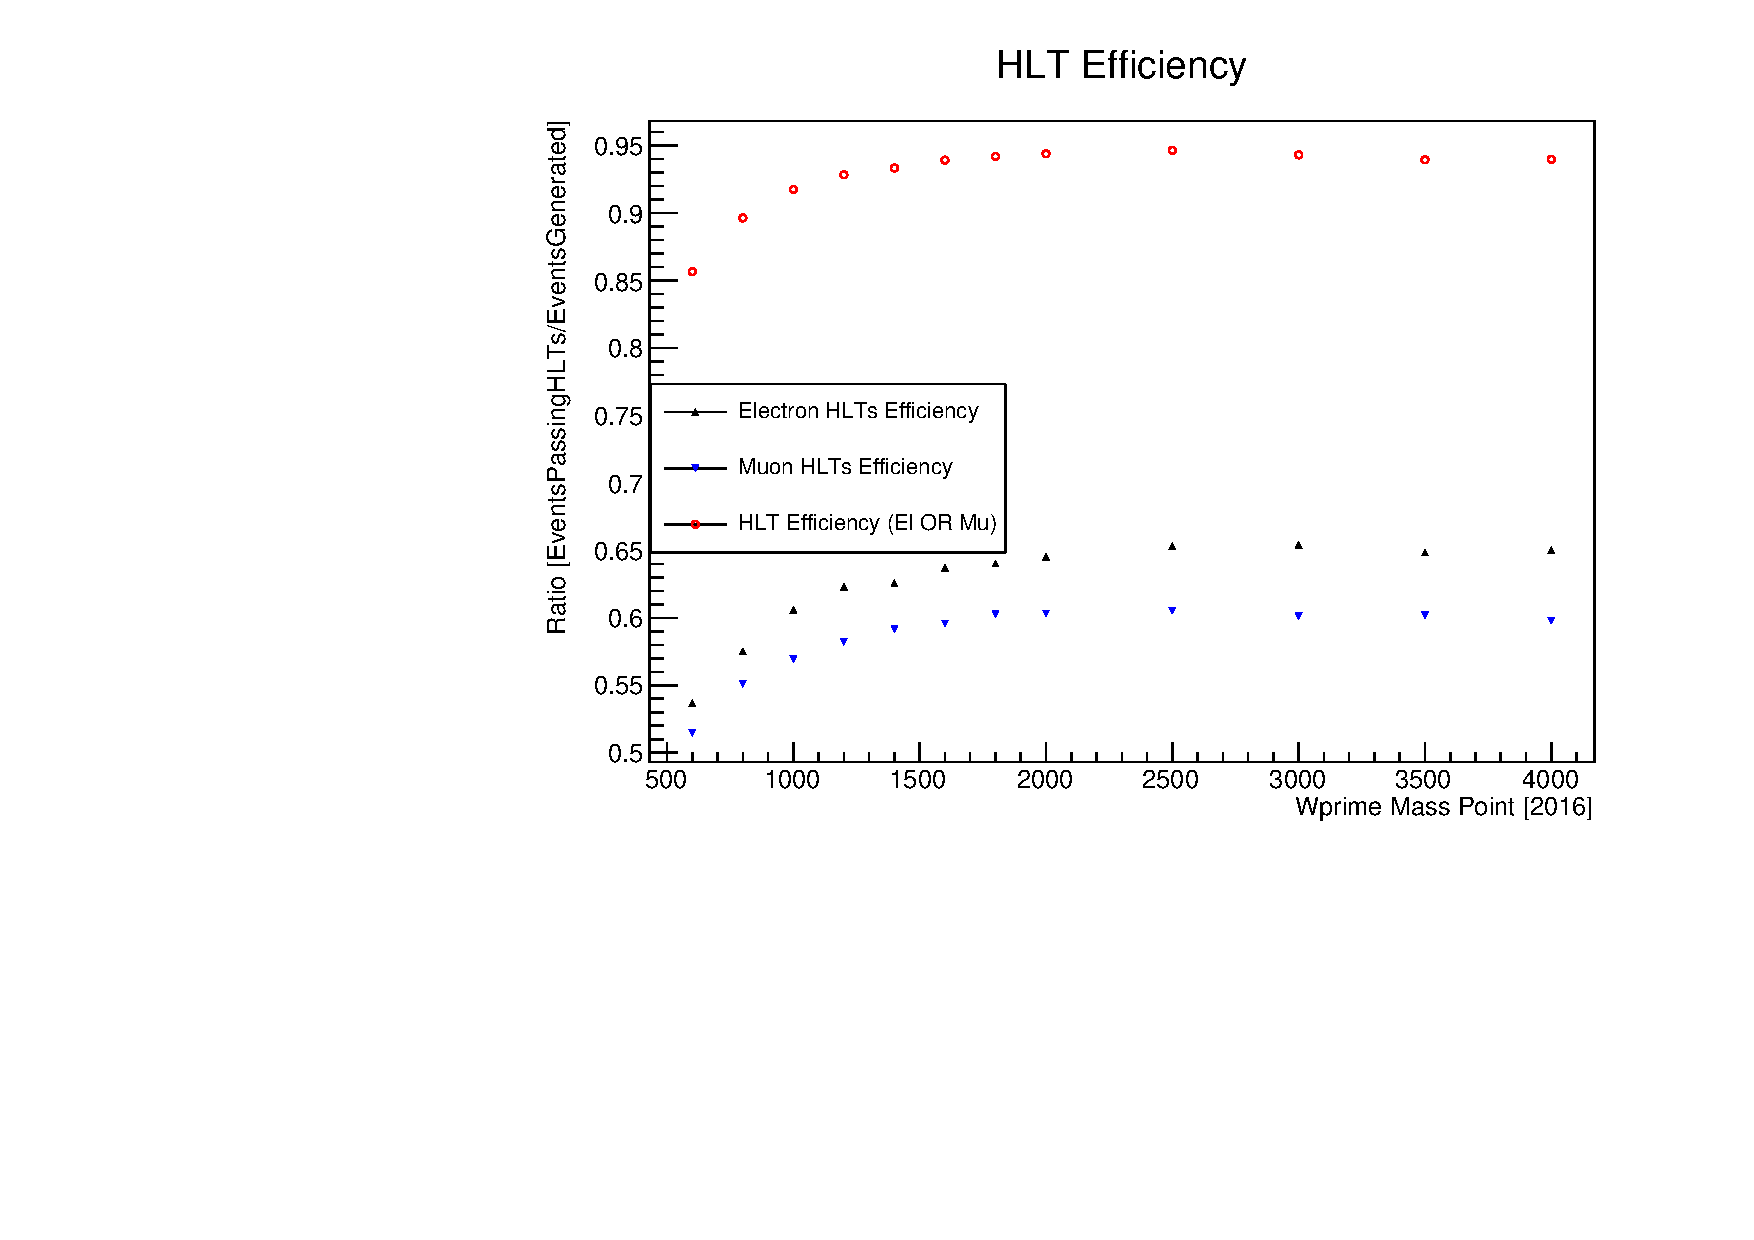
\includegraphics[width=.5\textwidth]{fig/2016_SignalTriggerEfficiency.pdf}}
        \subfigure[2017]{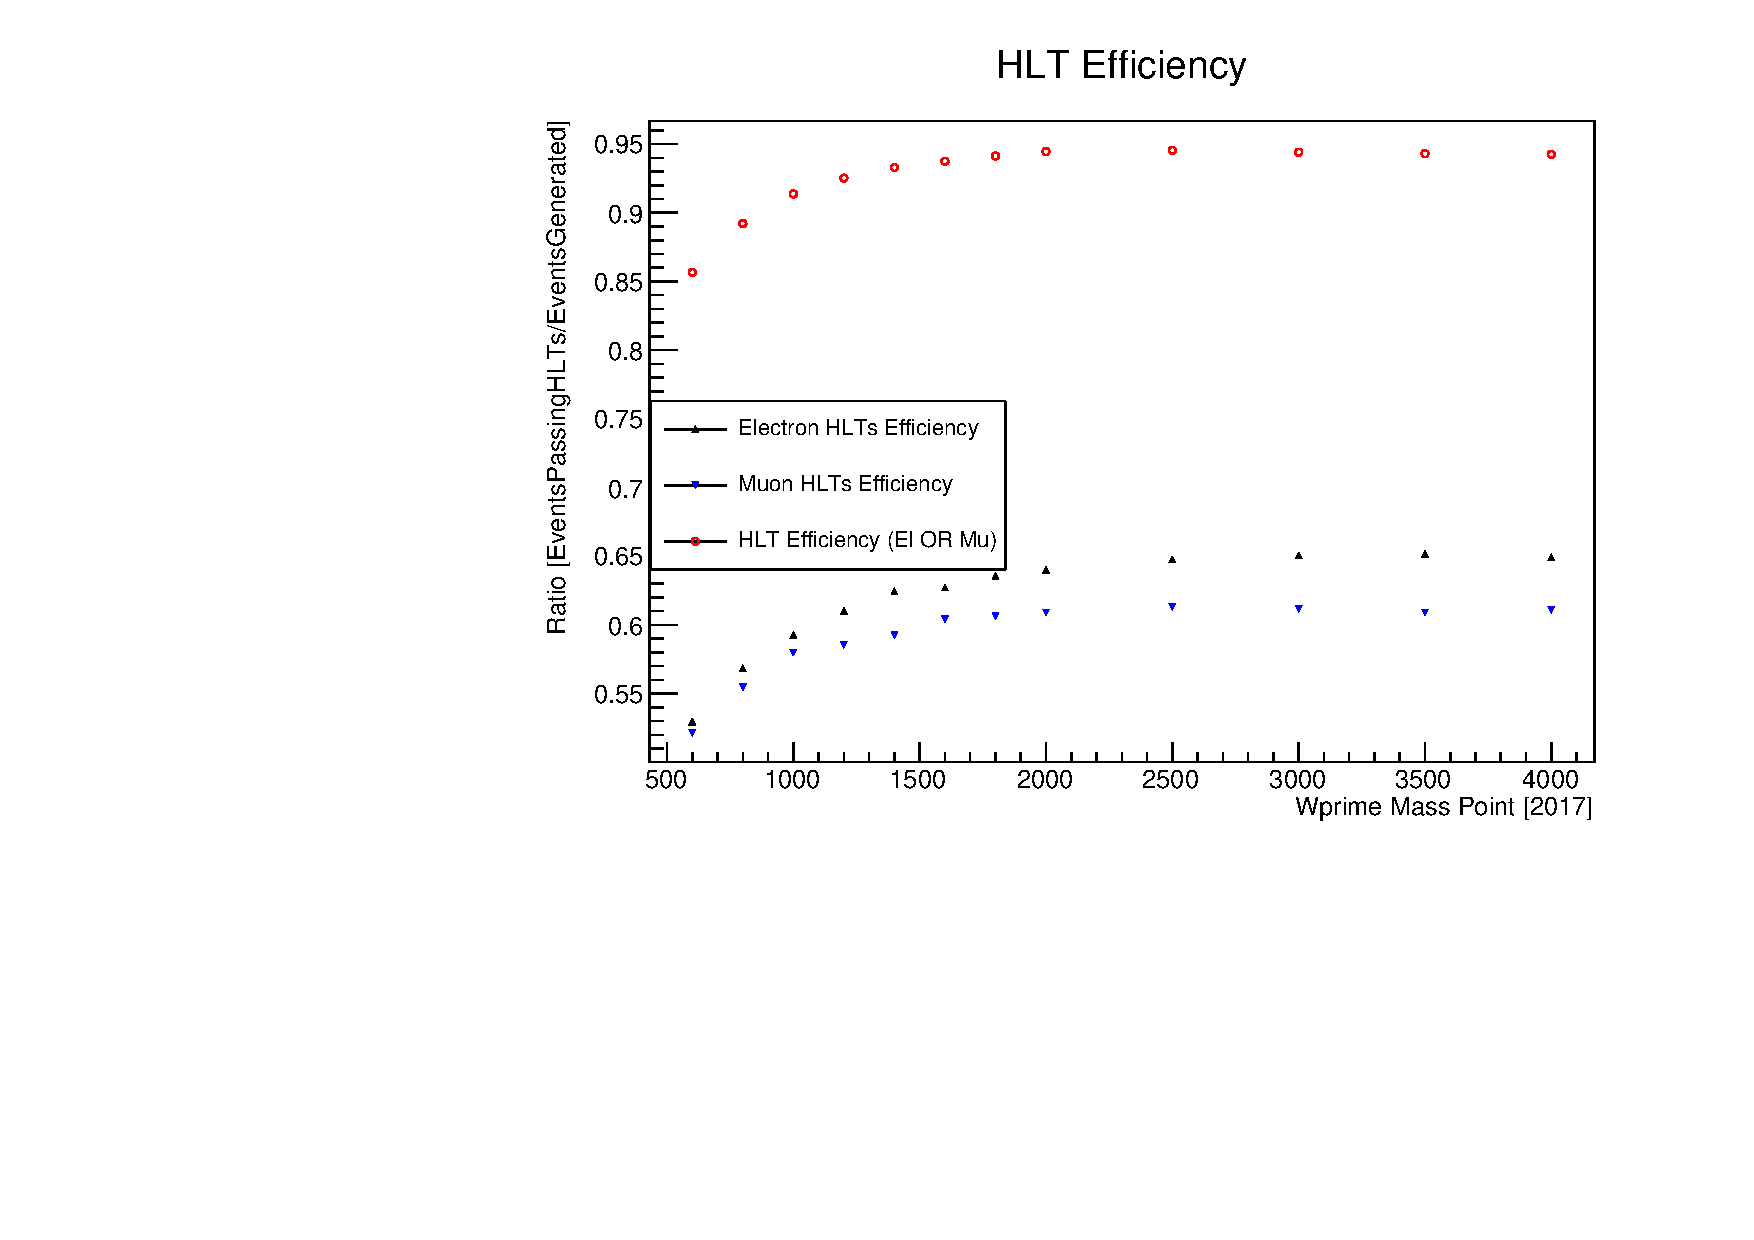
\includegraphics[width=.5\textwidth]{fig/2017_SignalTriggerEfficiency.pdf}}
        \vfil
        \subfigure[2018]{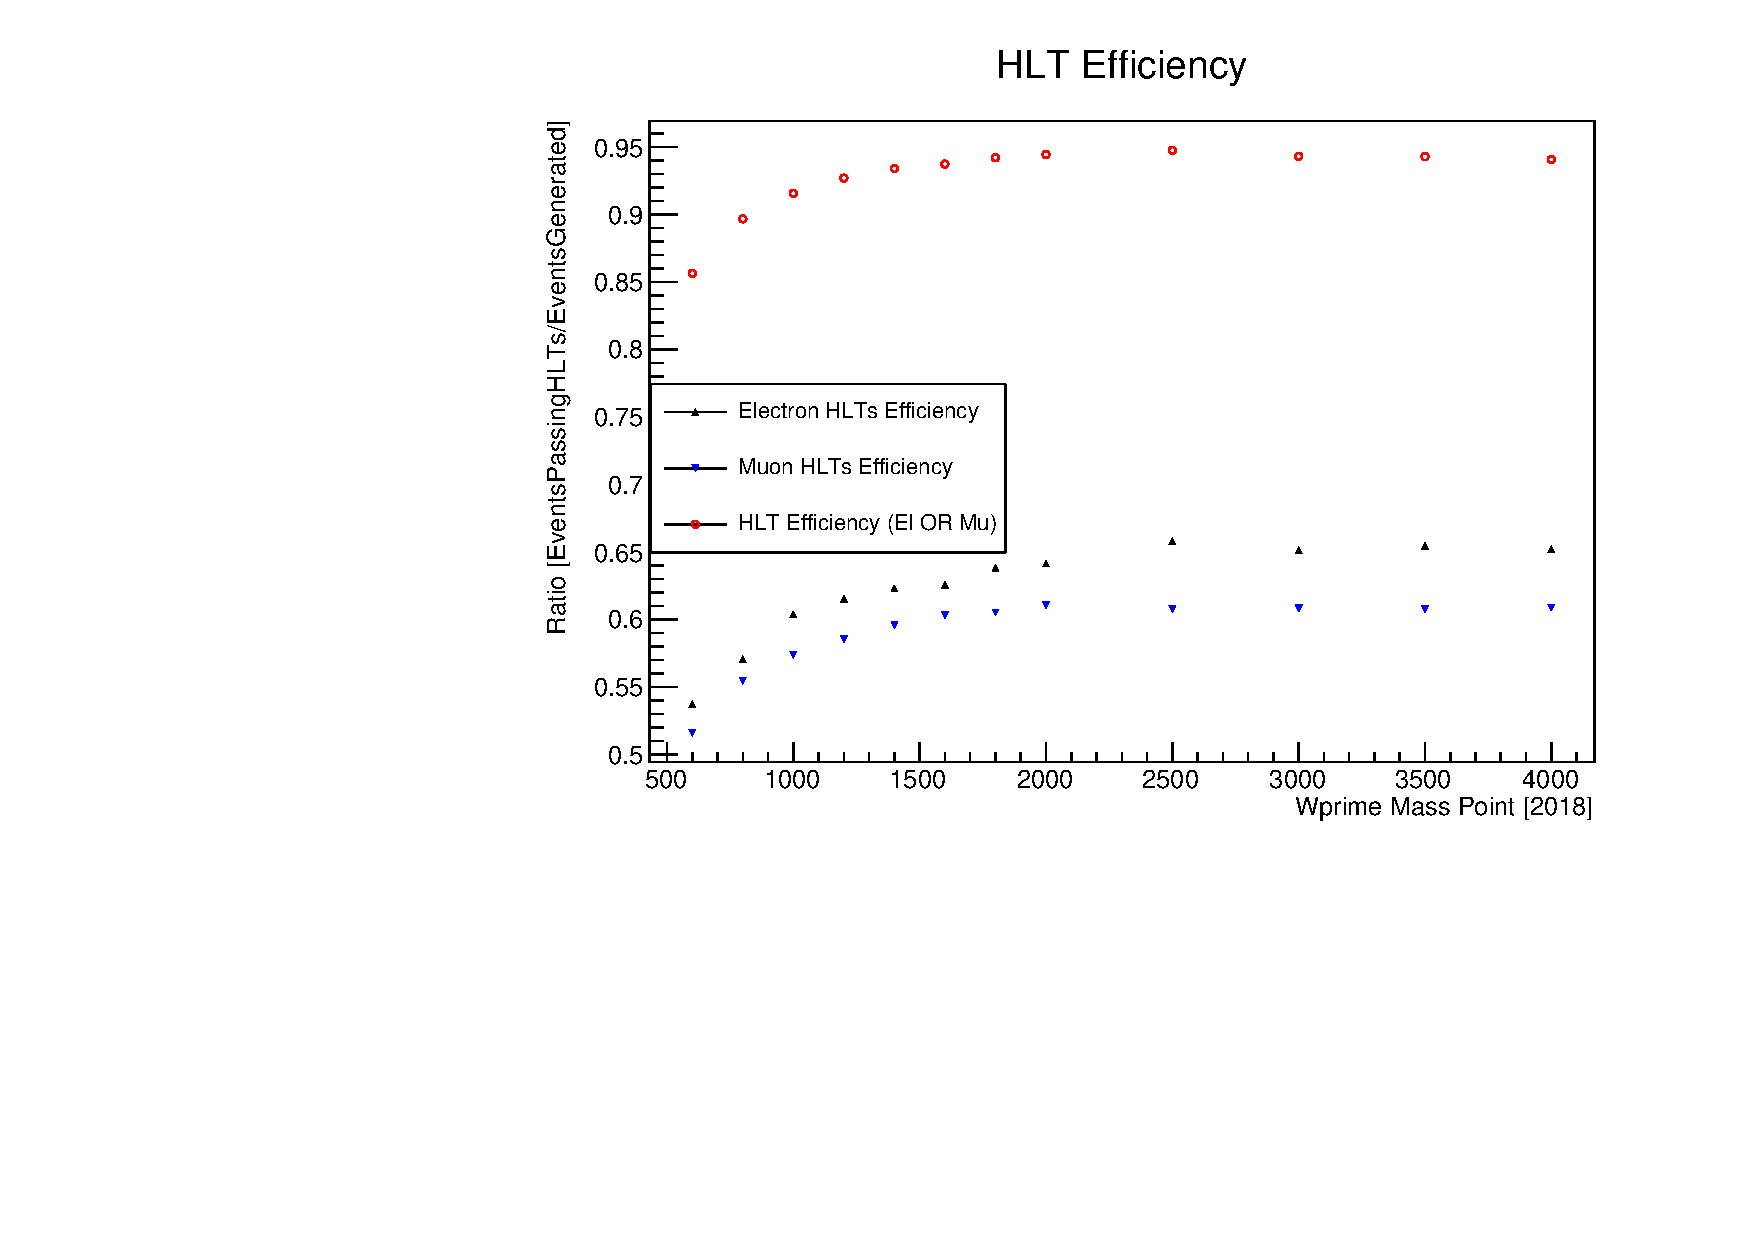
\includegraphics[width=.5\textwidth]{fig/2018_SignalTriggerEfficiency.pdf}}
  \caption{Signal efficiency for individual and combined High Level Triggers for Run II}
  \label{fig:hltSignalEfficiency}
\end{figure}

\begin{figure}[tph]
  \centering
  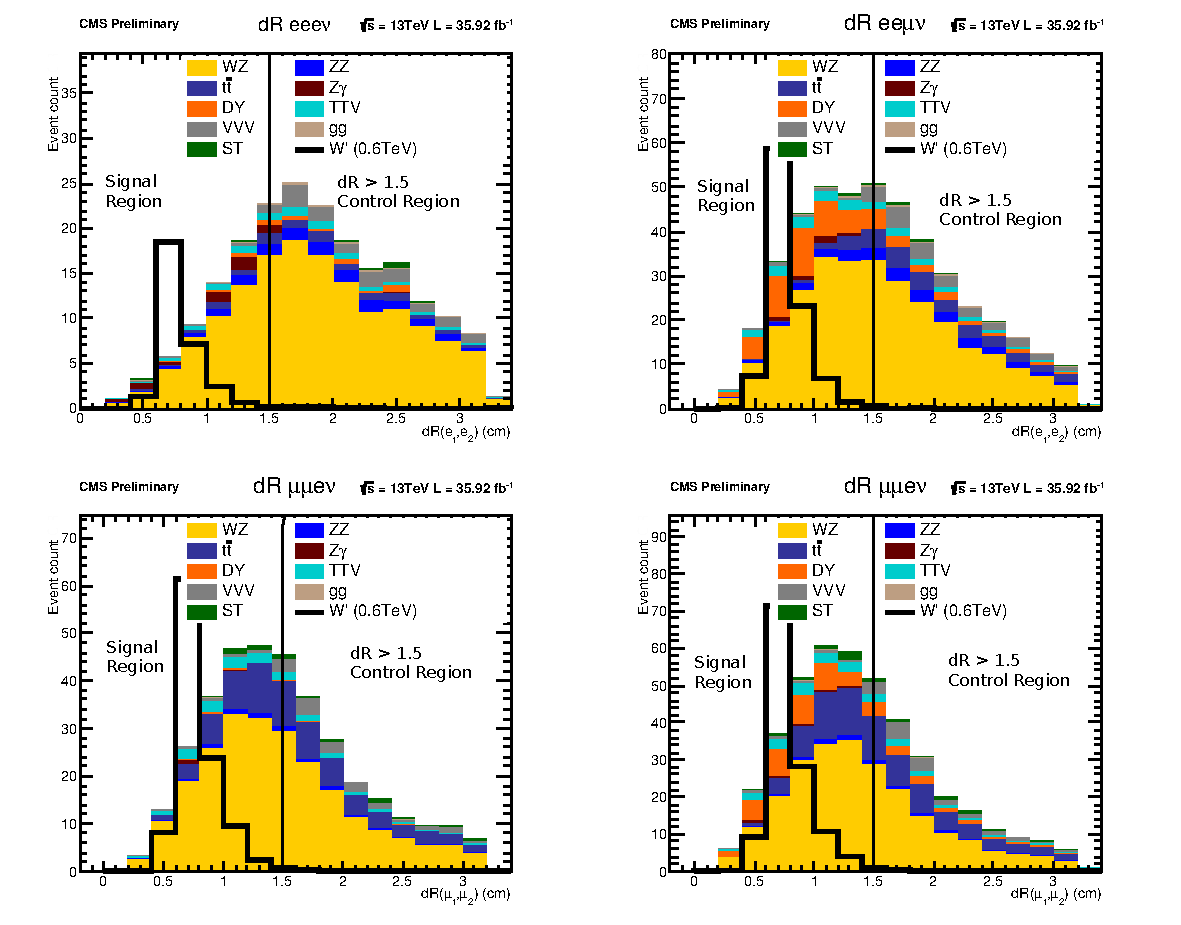
\includegraphics[width=\textwidth]{fig/Run2/KFactorIncluded_HDistl1l2_CR1_A+HDisM600.pdf}
  \caption{Definition of the signal and control regions. All the channels
    show how the region $dr_{l_{1}l_{2}} > 1.5$ is signal-depleted. A $600 GeV$
    mass resonance is used for illustration purposes. The larger the resonance
    mass, the narrower the signal distribution gets and it is shifted towards
    the lower $dR$ region as the leptons product of the $Z$ decay get closer
    forming a boosted topology.
    Top left: $Z(\rightarrow e+e)W(\rightarrow e+\nu)$
    Top right: $Z(\rightarrow e+e)W(\rightarrow \mu+\nu)$
    Bottom left: $Z(\rightarrow \mu+\mu)W(\rightarrow e+\nu)$
    Bottom right: $Z(\rightarrow \mu+\mu)W(\rightarrow \mu+\nu)$}
  \label{fig:ControlRegionDefinition}
\end{figure}

In order to analyse the simulation quality, the data/MC ratio is studied on
a signal-depleted control region. As Figure \ref{fig:ControlRegionDefinition}
shows, the distance in the $\eta-\phi$ plane between the products
of the Z boson decay $Z(\rightarrow l_{1}+l_{2})$ allow a distinct separation between a signal-enriched
region ($dr_{l_{1}l_{2}} <= 1.5$) and a signal depleted region
($dr_{l_{1}l_{2}} > 1.5$). The signal-delepted region is dominated mainly by
the SM WZ production process.

\begin{figure}[tph]
  \centering
  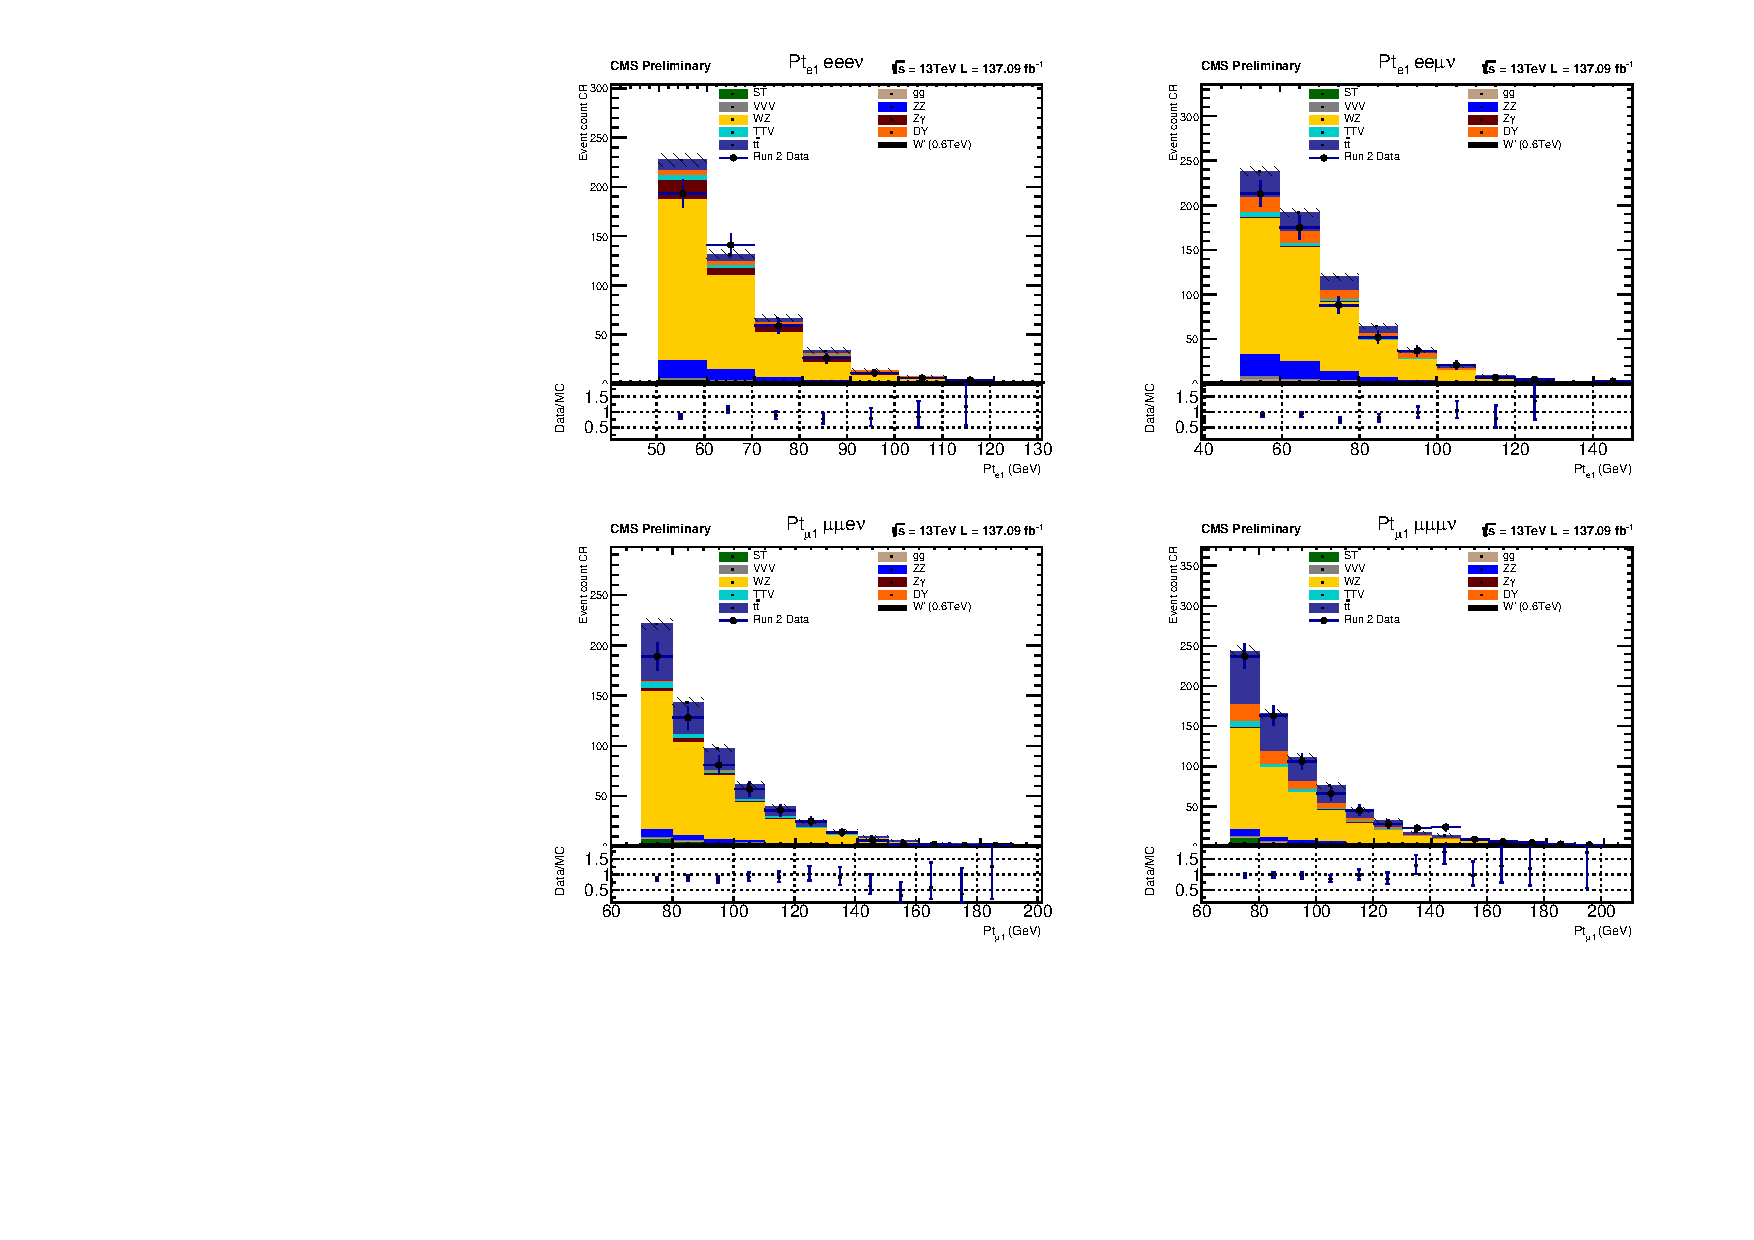
\includegraphics[width=\textwidth]{fig/Run2/KFactorIncluded_HPtl1_CR1_A_Run2_HPtRun2_M600.pdf}
  \caption{Leading lepton transverse momentum distributions for each final
    signature as seen in the $dr_{l_{1}l_{2}} > 1.5$ control region.
    Top left: $Z(\rightarrow e+e)W(\rightarrow e+\nu)$
    Top right: $Z(\rightarrow e+e)W(\rightarrow \mu+\nu)$
    Bottom left: $Z(\rightarrow \mu+\mu)W(\rightarrow e+\nu)$
    Bottom right: $Z(\rightarrow \mu+\mu)W(\rightarrow \mu+\nu)$}
  \label{fig:CR1_Run2_HPtl1}
\end{figure}

\begin{figure}[tph]
  \centering
  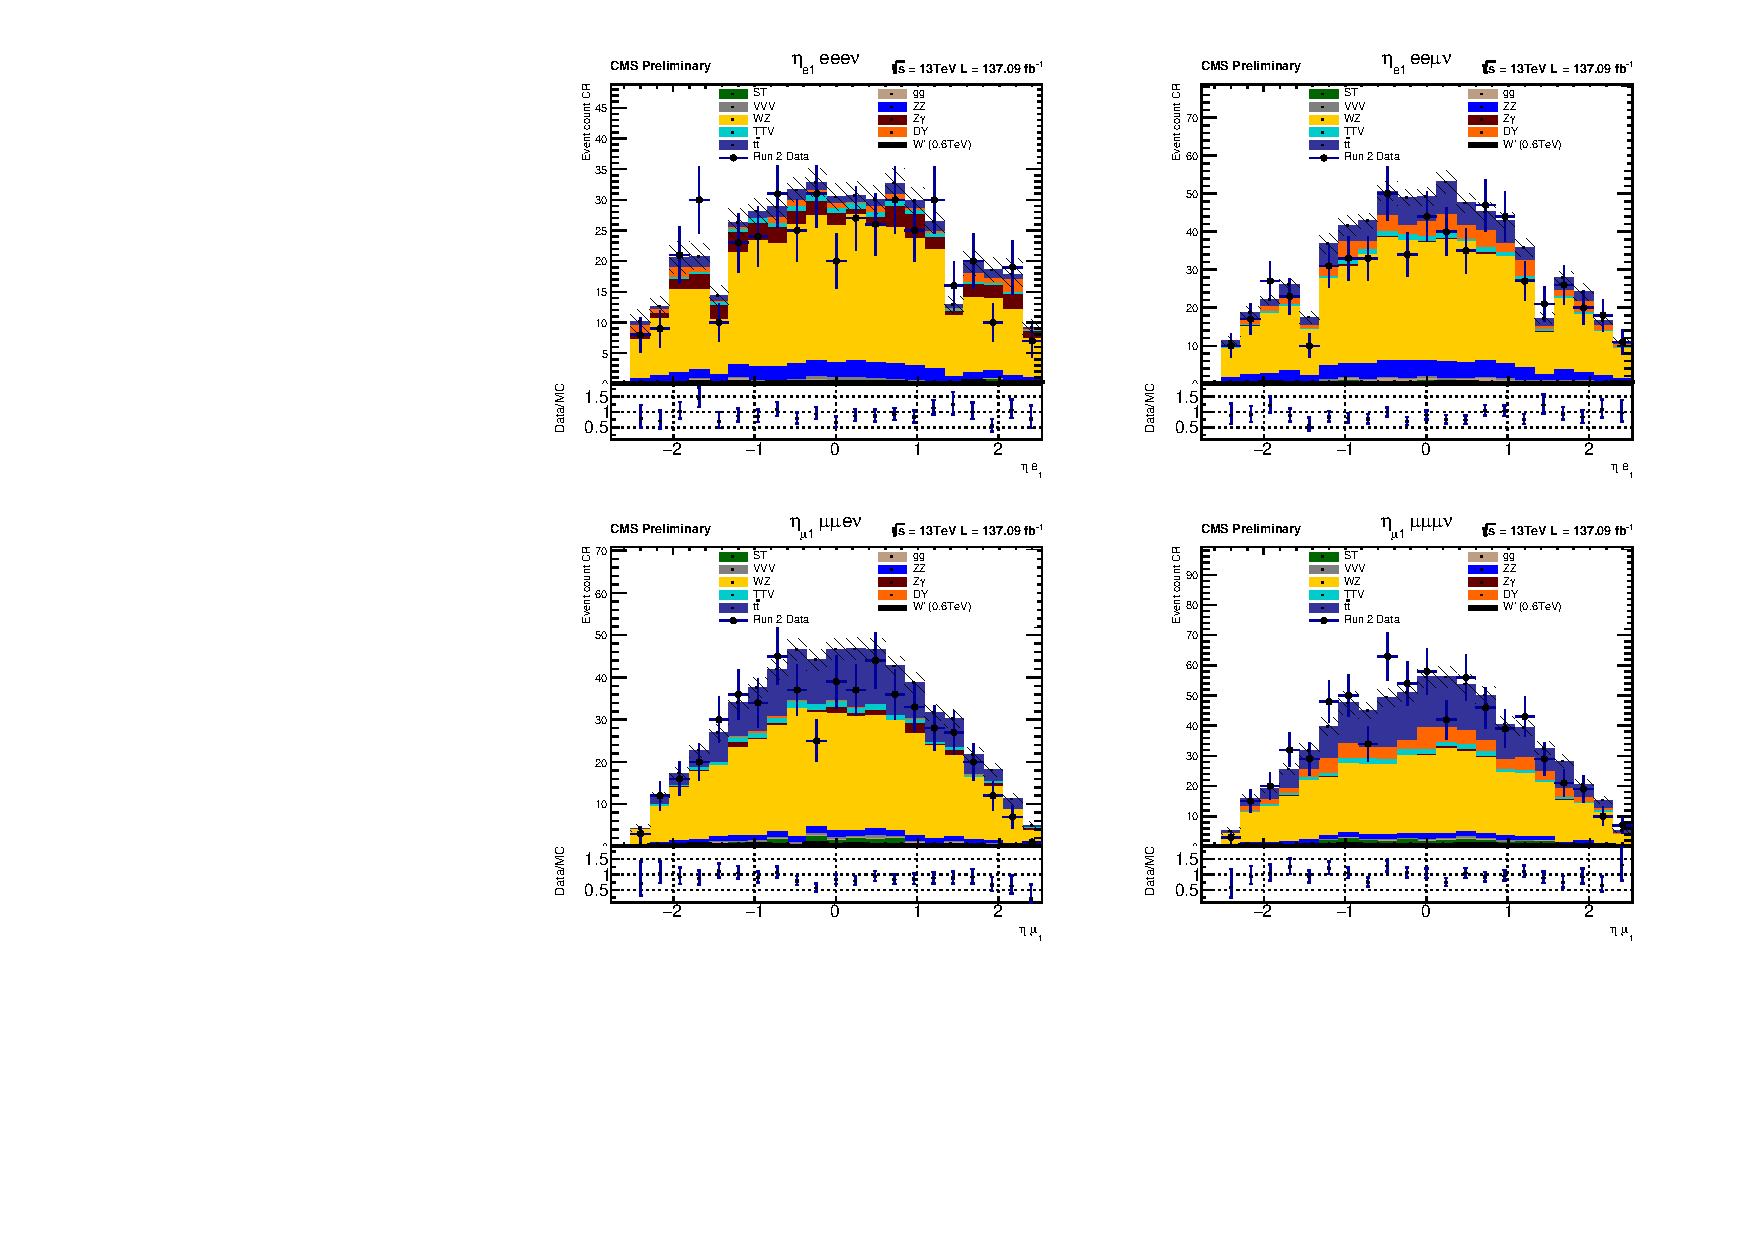
\includegraphics[width=\textwidth]{fig/Run2/KFactorIncluded_HEtal1_CR1_A_Run2_HERun2_M600.pdf}
  \caption{Leading lepton $\eta$ distributions for each final
    signature as seen in the $dr_{l_{1}l_{2}} > 1.5$ control region.
    Top left: $Z(\rightarrow e+e)W(\rightarrow e+\nu)$
    Top right: $Z(\rightarrow e+e)W(\rightarrow \mu+\nu)$
    Bottom left: $Z(\rightarrow \mu+\mu)W(\rightarrow e+\nu)$
    Bottom right: $Z(\rightarrow \mu+\mu)W(\rightarrow \mu+\nu)$}
  \label{fig:CR1_Run2_HEtal1}
\end{figure}

\begin{figure}[tph]
  \centering
  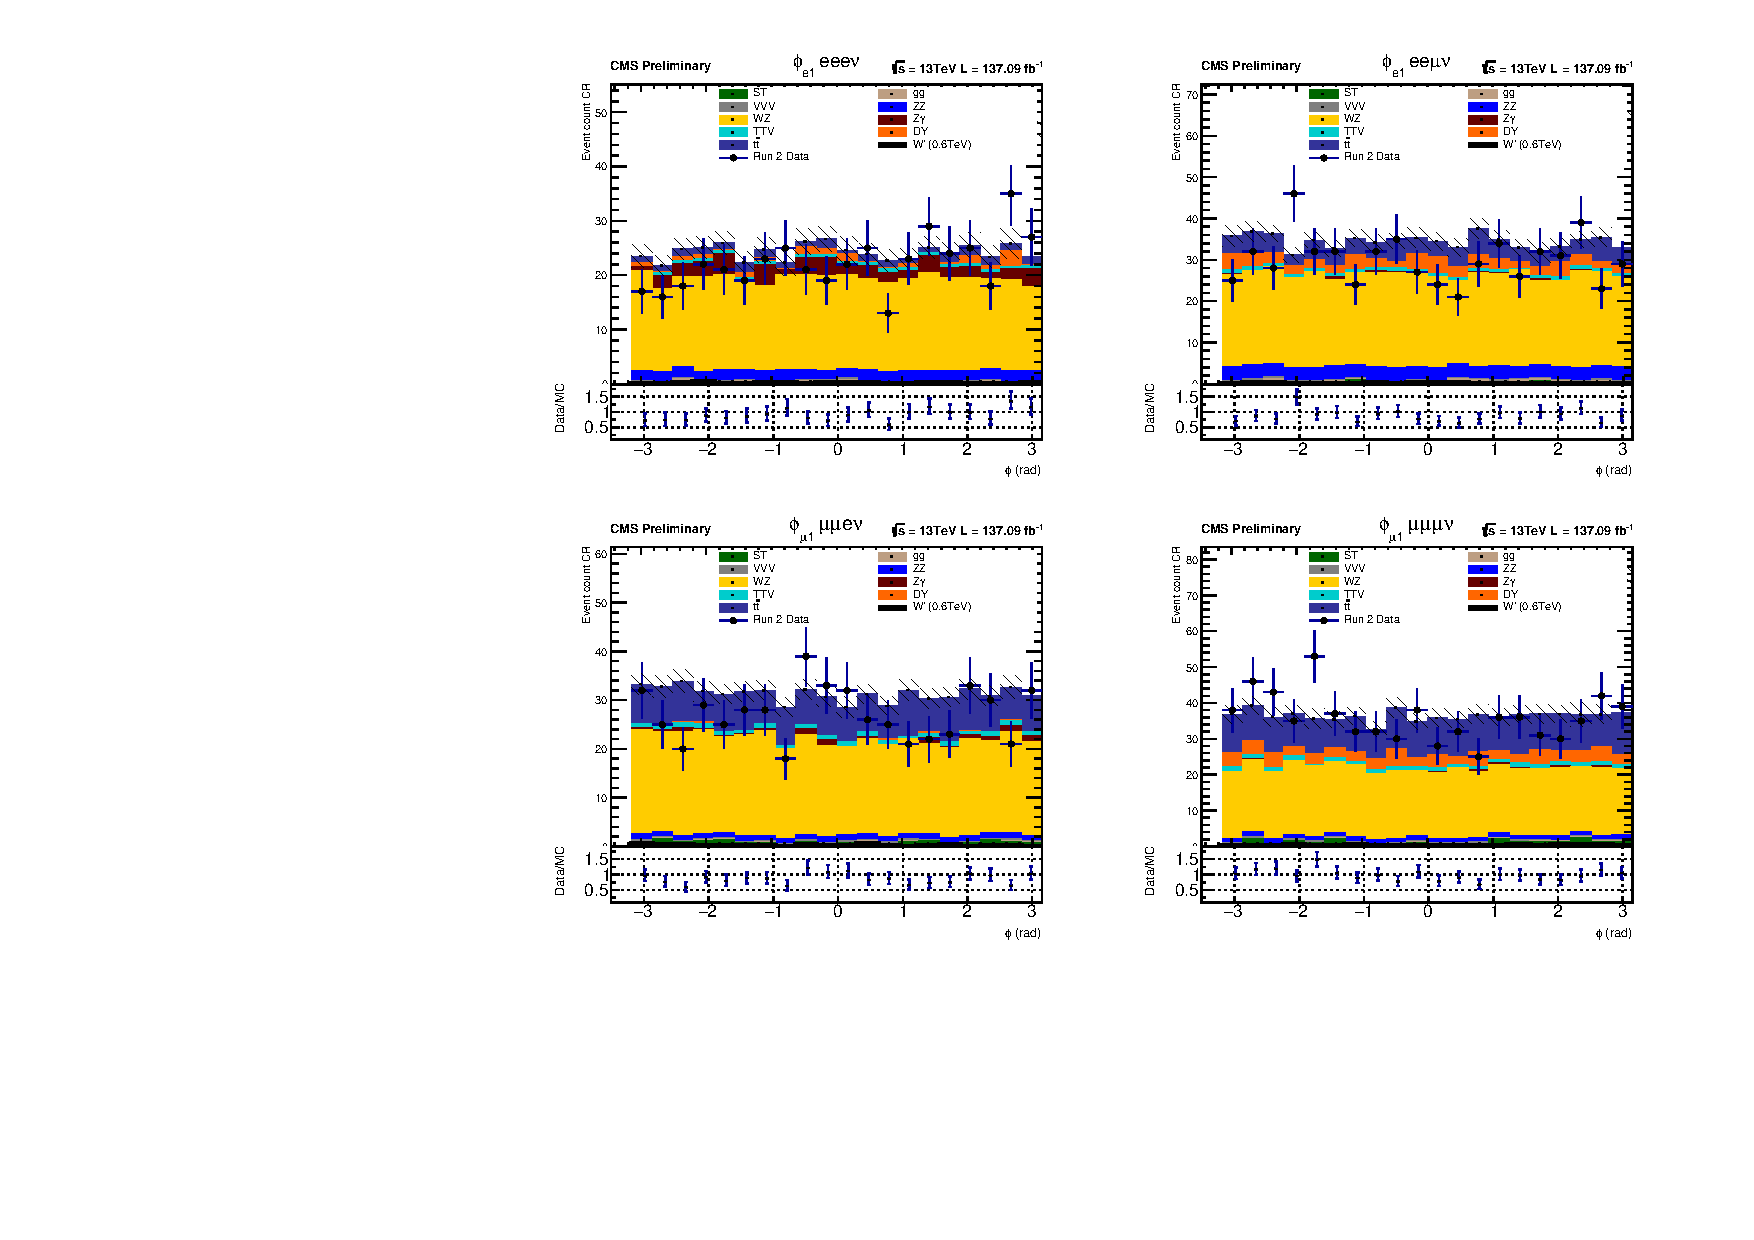
\includegraphics[width=\textwidth]{fig/Run2/KFactorIncluded_HPhil1_CR1_A_Run2_HPRun2_M600.pdf}
  \caption{Leading lepton $phi$ distributions for each final
    signature as seen in the $dr_{l_{1}l_{2}} > 1.5$ control region.
    Top left: $Z(\rightarrow e+e)W(\rightarrow e+\nu)$
    Top right: $Z(\rightarrow e+e)W(\rightarrow \mu+\nu)$
    Bottom left: $Z(\rightarrow \mu+\mu)W(\rightarrow e+\nu)$
    Bottom right: $Z(\rightarrow \mu+\mu)W(\rightarrow \mu+\nu)$}
  \label{fig:CR1_Run2_HPhil1}
\end{figure}

\begin{figure}[tph]
  \centering
  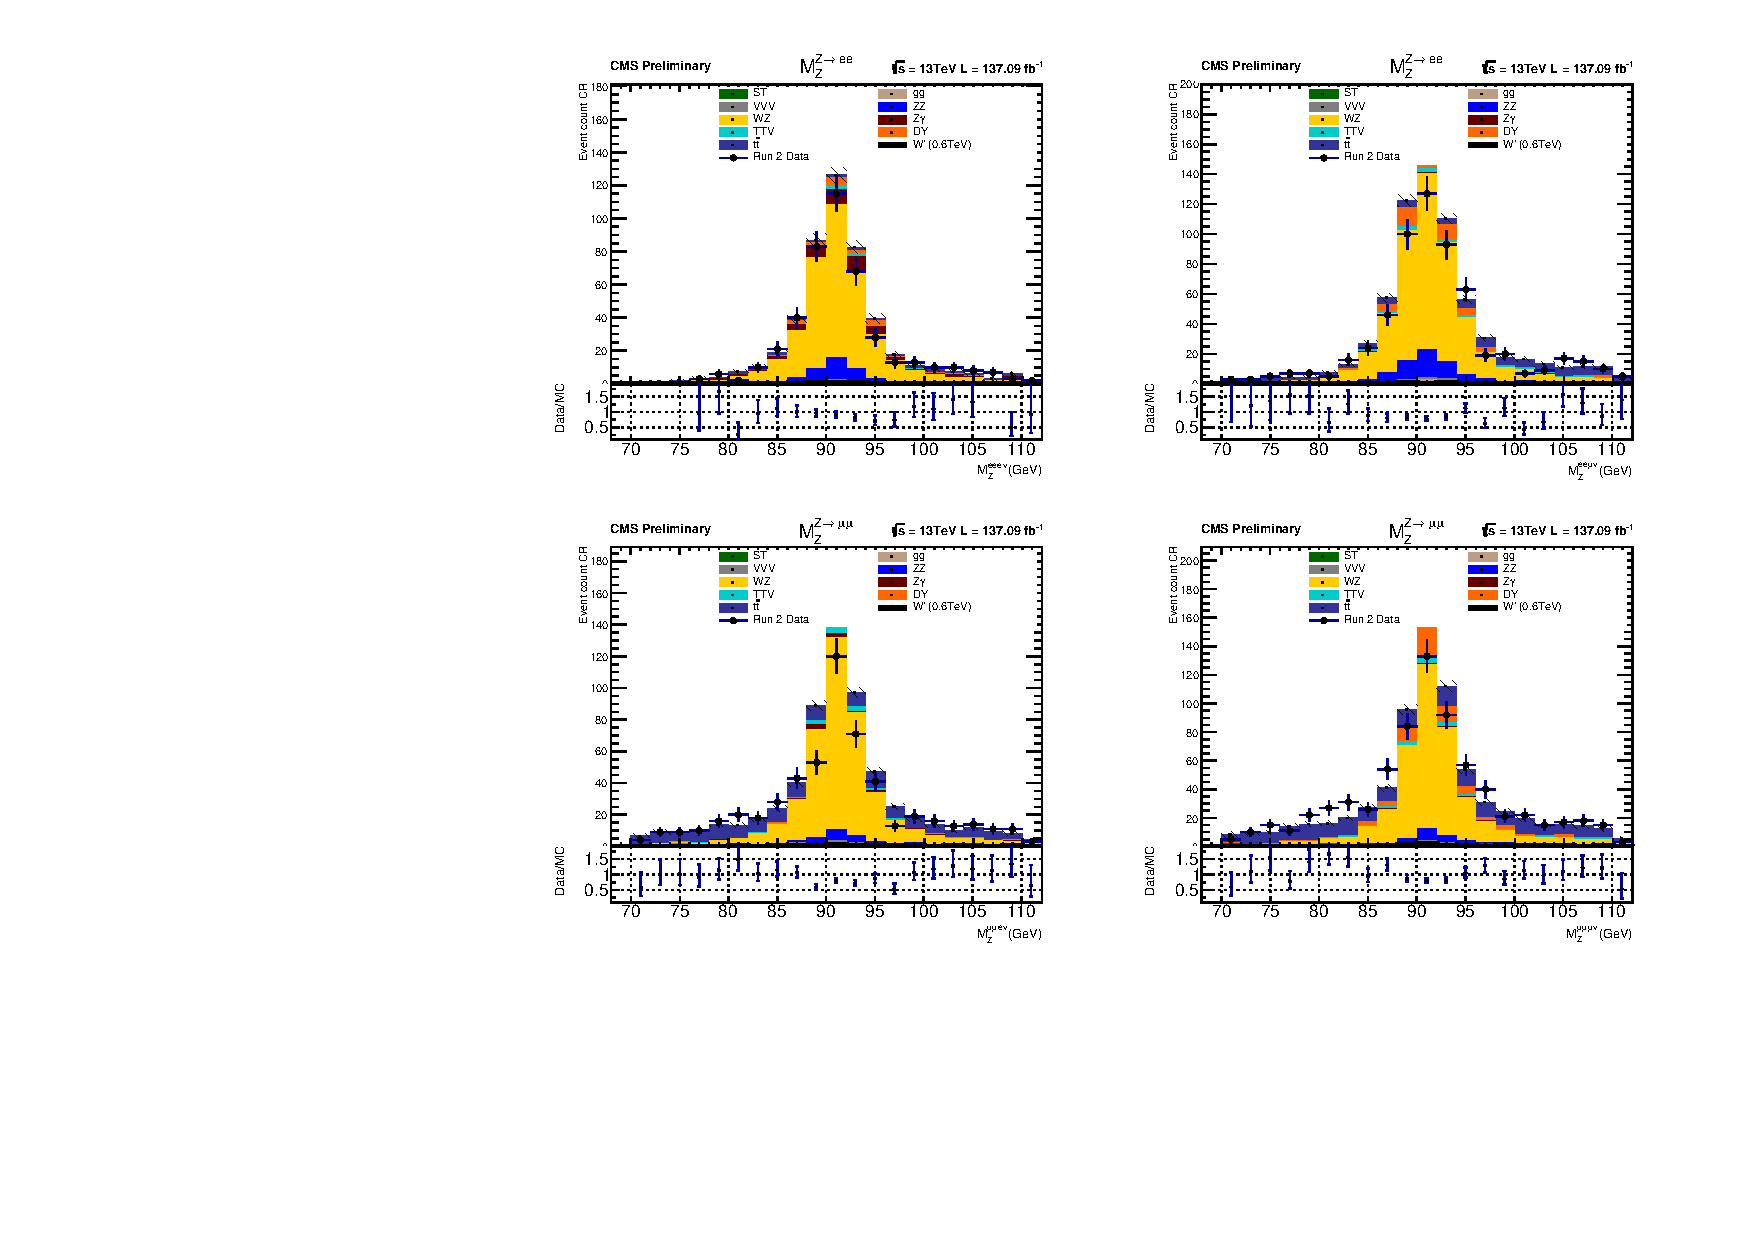
\includegraphics[width=\textwidth]{fig/Run2/KFactorIncluded_HMassZ_CR1_A_Run2_HMRun2_M600.pdf}
  \caption{$M_{Z}$ distributions of $Z\rightarrow\ell\ell$ candidates for each final
    signature as seen in the $dr_{l_{1}l_{2}} > 1.5$ control region.
    Top left: $Z(\rightarrow e+e)W(\rightarrow e+\nu)$
    Top right: $Z(\rightarrow e+e)W(\rightarrow \mu+\nu)$
    Bottom left: $Z(\rightarrow \mu+\mu)W(\rightarrow e+\nu)$
    Bottom right: $Z(\rightarrow \mu+\mu)W(\rightarrow \mu+\nu)$}
  \label{fig:CR1_Run2_HMassZ}
\end{figure}

\begin{figure}[tph]
  \centering
  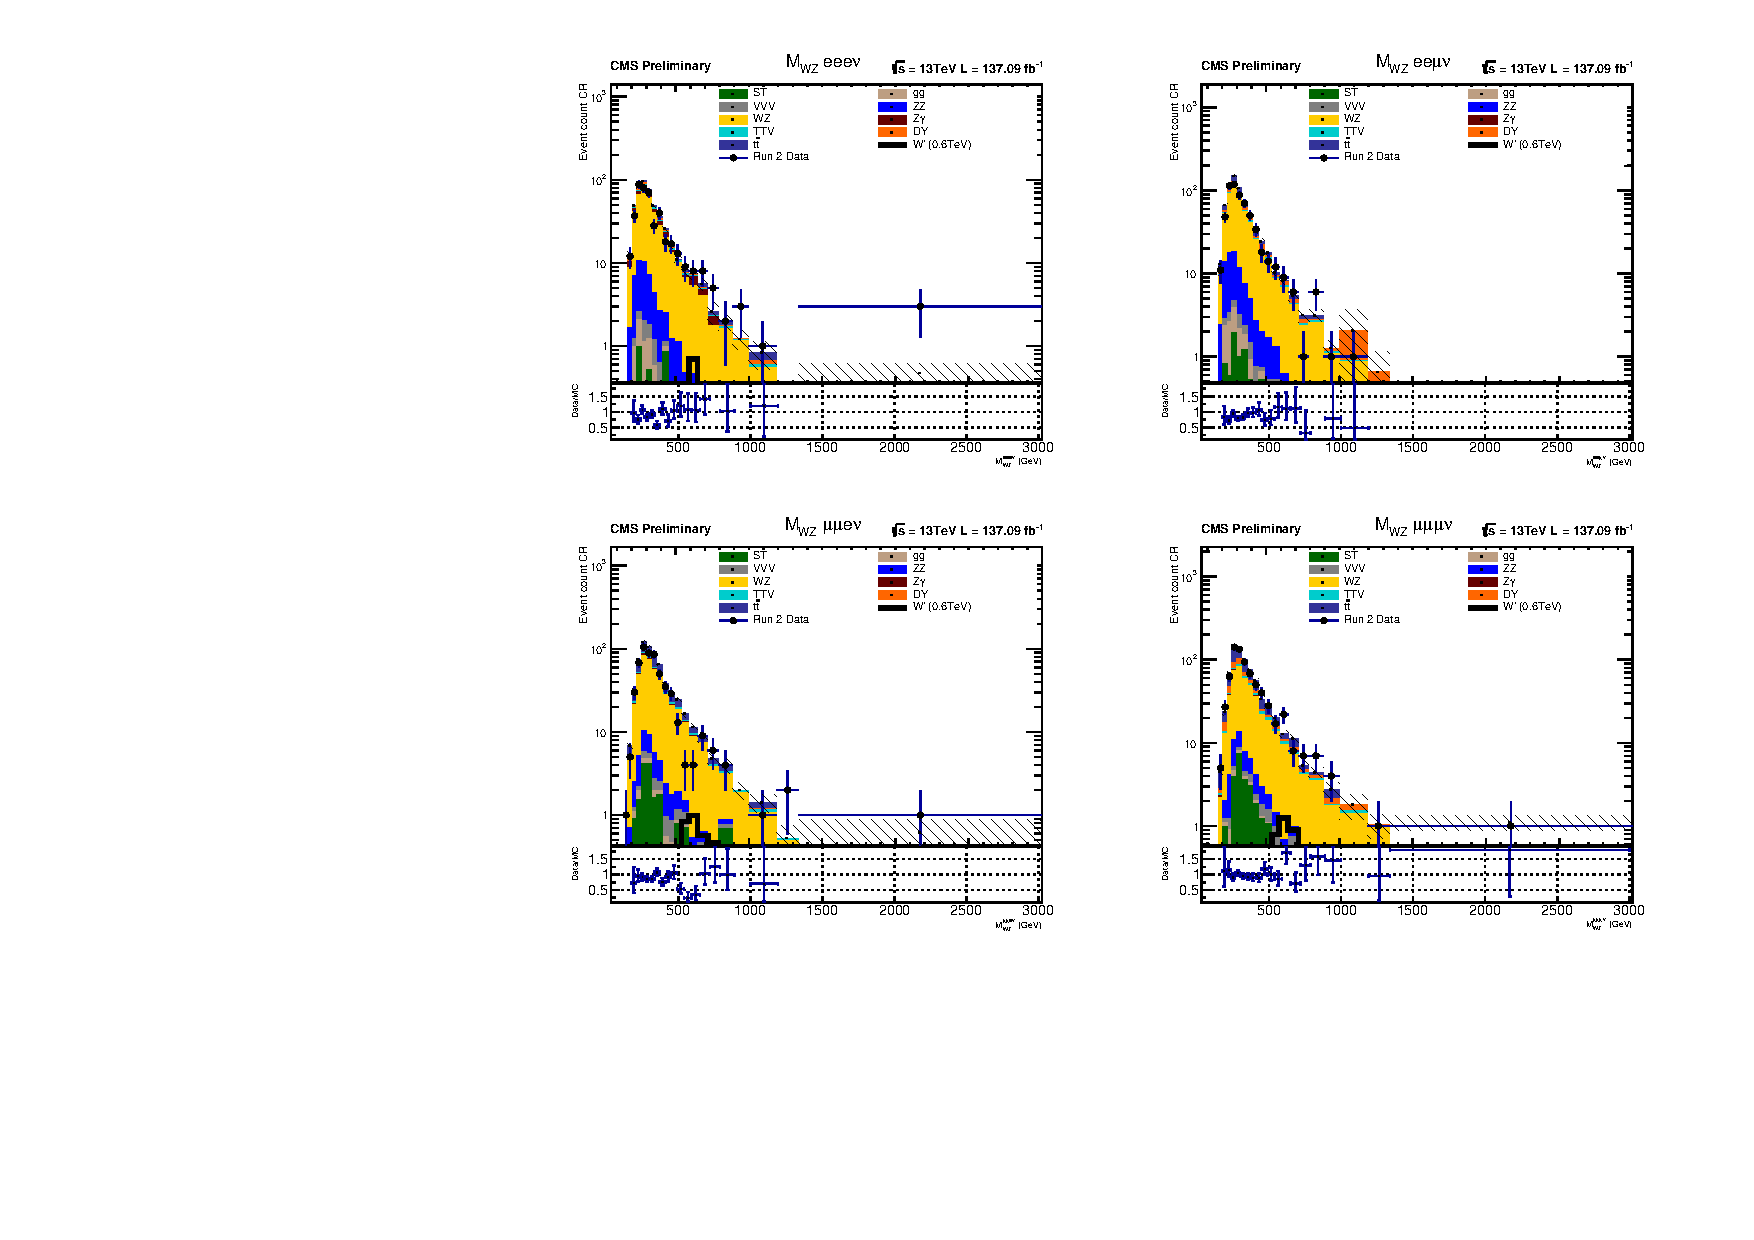
\includegraphics[width=\textwidth]{fig/Run2/Rebining_HMassWZ_CR1_A_Run2_HRun2_M600.pdf}
  \caption{The $WZ$ invariant mass after the $WZ$ candidate selection for each final
    signature as seen in the $dr_{l_{1}l_{2}} > 1.5$ control region.
    Top left: $Z(\rightarrow e+e)W(\rightarrow e+\nu)$
    Top right: $Z(\rightarrow e+e)W(\rightarrow \mu+\nu)$
    Bottom left: $Z(\rightarrow \mu+\mu)W(\rightarrow e+\nu)$
    Bottom right: $Z(\rightarrow \mu+\mu)W(\rightarrow \mu+\nu)$}
  \label{fig:CR1_Run2_HMassWZ}
\end{figure}

\begin{figure}[tph]
  \centering
  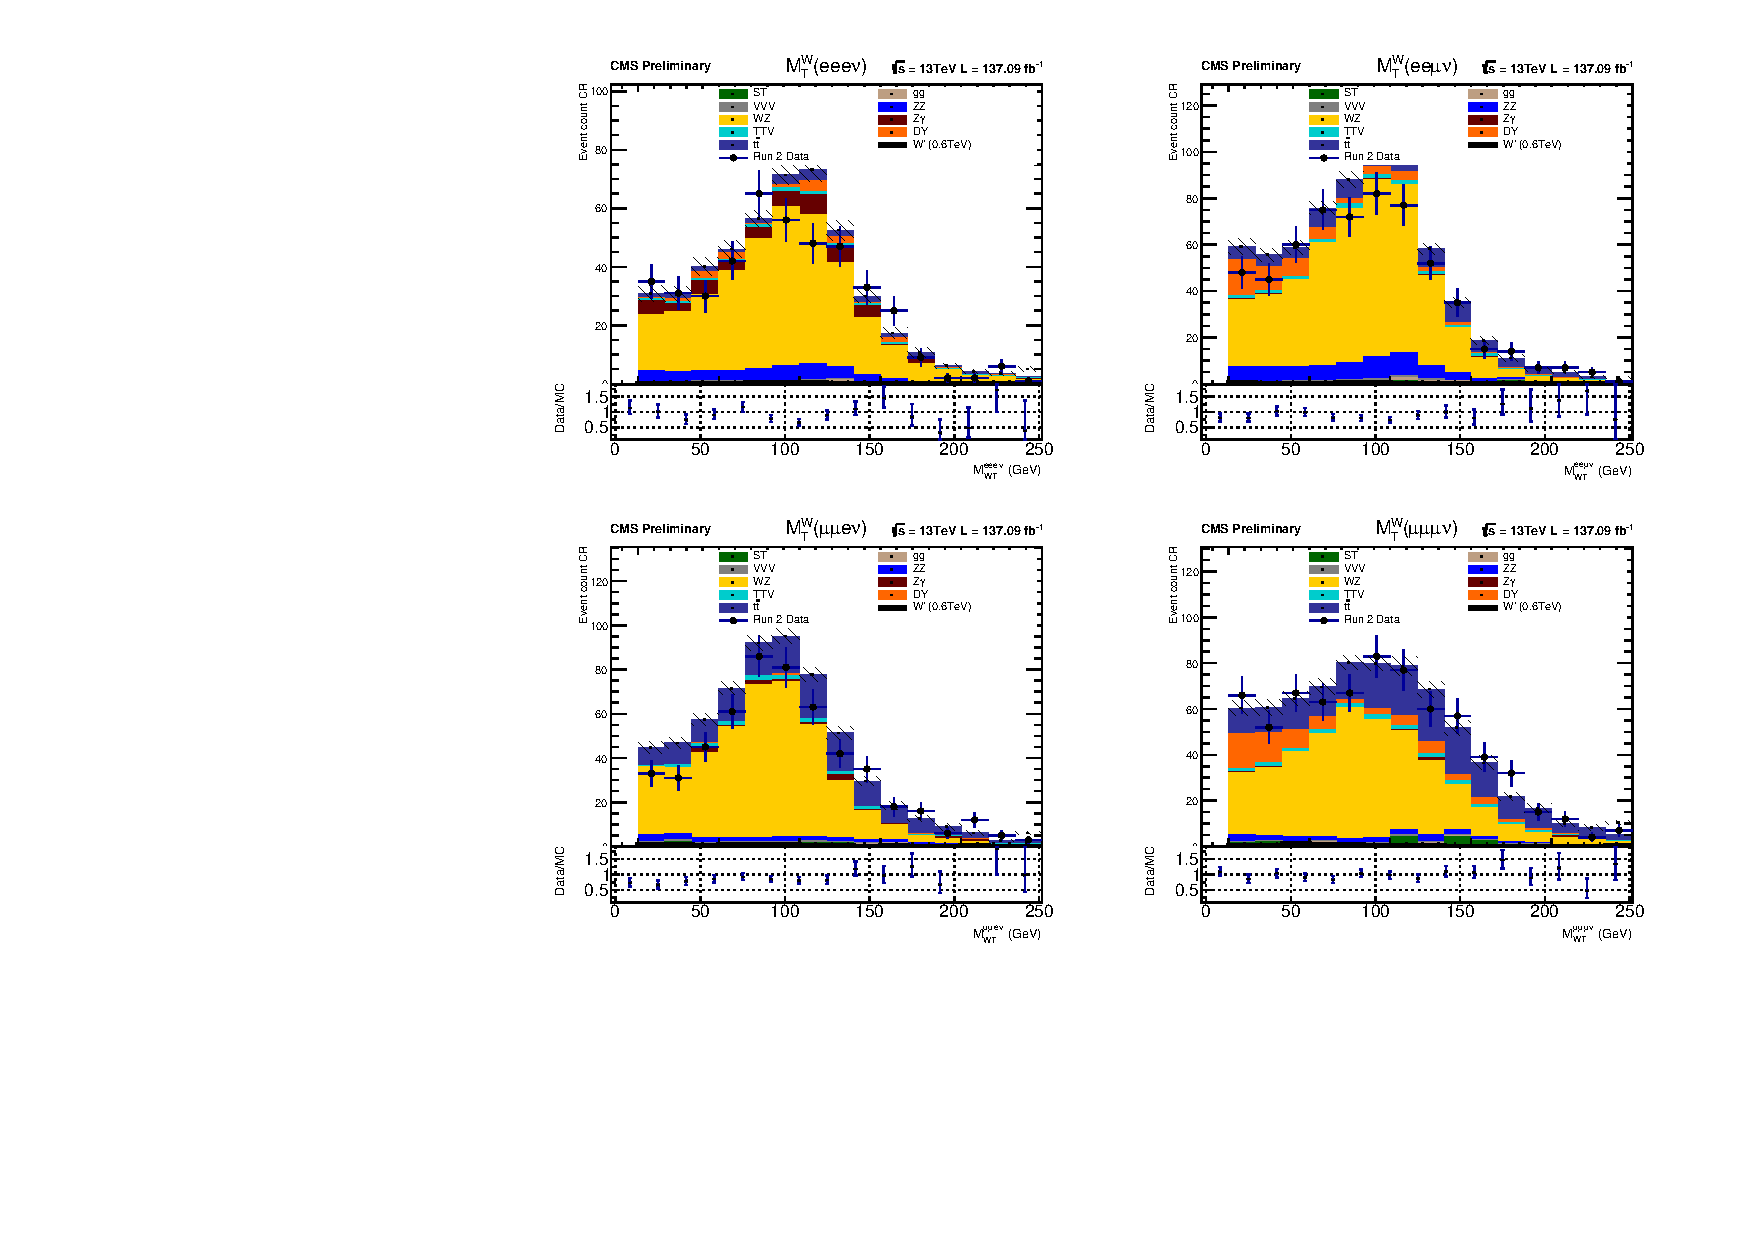
\includegraphics[width=\textwidth]{fig/Run2/KFactorIncluded_HMassTW_CR1_A_Run2_HRun2_M600.pdf}
  \caption{The transverse mass distribution for the $W$ candidate for each final
    signature as seen in the $dr_{l_{1}l_{2}} > 1.5$ control region.
    Top left: $Z(\rightarrow e+e)W(\rightarrow e+\nu)$
    Top right: $Z(\rightarrow e+e)W(\rightarrow \mu+\nu)$
    Bottom left: $Z(\rightarrow \mu+\mu)W(\rightarrow e+\nu)$
    Bottom right: $Z(\rightarrow \mu+\mu)W(\rightarrow \mu+\nu)$}
  \label{fig:CR1_Run2_HMassTW}
\end{figure}

The $\eta$, $\phi$, $P_{T}$ distributions for the leading lepton en each category
are shown in figures \ref{fig:CR1_Run2_HEtal1}, \ref{fig:CR1_Run2_HPhil1}, and
\ref{fig:CR1_Run2_HPtl1}, as well as composite distributions like the mass of the
reconstructed Z candidate (Figure \ref{fig:CR1_Run2_HMassZ}), the $W$ boson transverse mass
(Figure \ref{fig:CR1_Run2_HMassTW}) and the discriminant variable: the mass for the
reconstructed diboson system (Figure \ref{fig:CR1_Run2_HMassWZ}) show a good data/MC
agreement in the control region.


\section{Corrections on MC}

\subsection{Luminosity Scale factors}

\begin{table}
  \caption{Run 2 Luminosity}
 \begin{center}
 \begin{tabular}{cc}\hline\hline
 Year & Luminosity [$fb^{-1}$] \\ \hline\hline
 2016 & 35.92  \\
 2017 & 41.43 \\
 2018 & 59.74 \\
 \end{tabular}
 \end{center}
 \label{tab:LuminosityPerYear}
\end{table}

The number of generated MC events listed on tables \ref{tab:BkgList2016}, \ref{tab:BkgList2017},
and \ref{tab:BkgList2018} are arbitrary. In order to compare it with data, the
former has to be rescaled to account for the amount of data collected each year
during the data taking period. The luminosity scale factor is computed as follows:

\begin{equation}
  L_{sf}=\frac{L_{\rm data}}{L_{\rm MC}} = \frac{L_{\rm data}\times\sigma_{\rm MC}}{n_{\rm MC}},
\label{eq:lumiSF}
\end{equation}

Where $L_{\rm data}$ is the luminosity per year, see table \ref{tab:LuminosityPerYear},
$n_{MC}$ the number of generated MC events as provided by the sum of weighted events
from the generator (\verb|genWeight| branch on \verb|NanoAOD|), and $\sigma_{\rm MC}$
is the cross section of the MC samples as provided by \verb|XSecAnalyzer|.

\subsection{Pileup Reweighting}

\begin{figure}[tph]
  \centering
        \subfigure[Standard model WZ production MC simulations normalized pileup distributions]{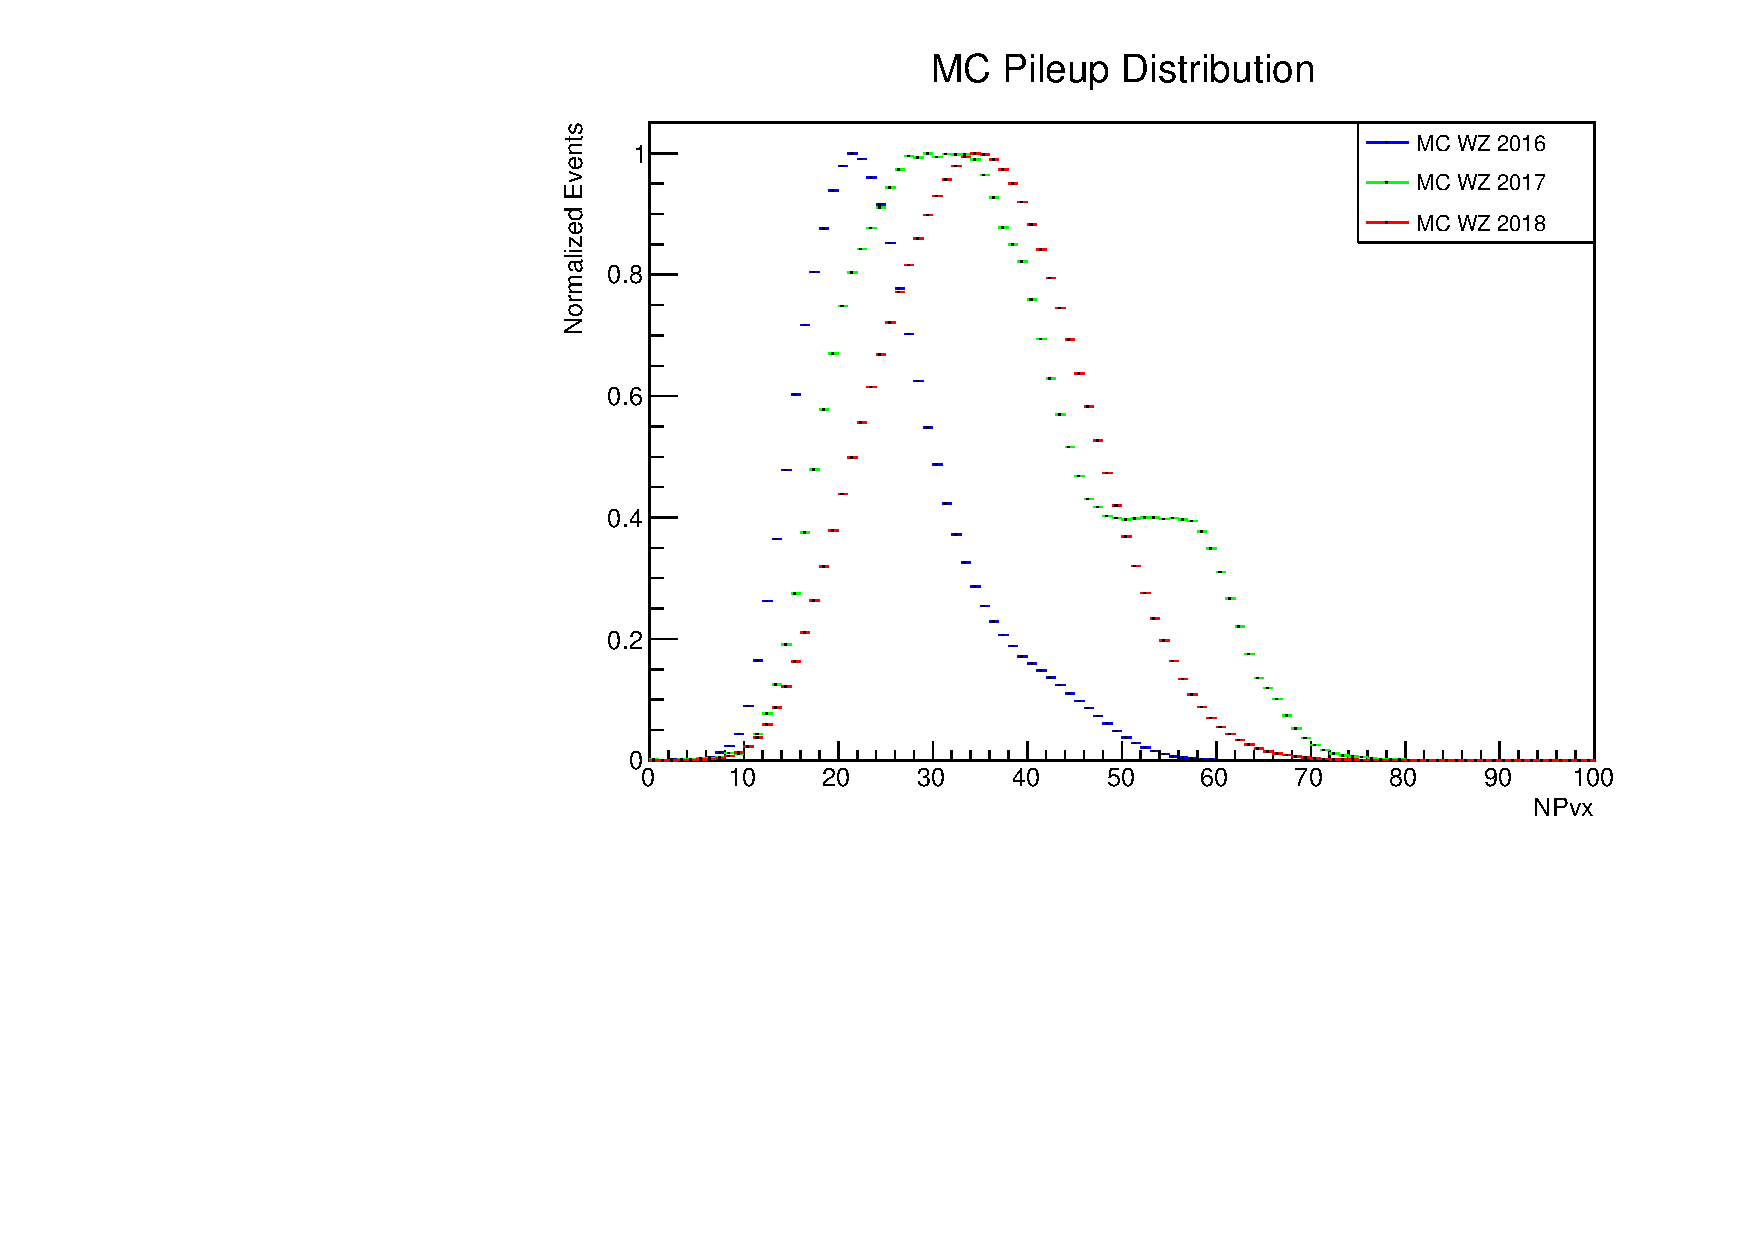
\includegraphics[width=.5\textwidth]{fig/ScaleFactors/MC_Pileup_Linear.pdf}}
        \subfigure[Pileup profile from RunII Data, Linear Scale]{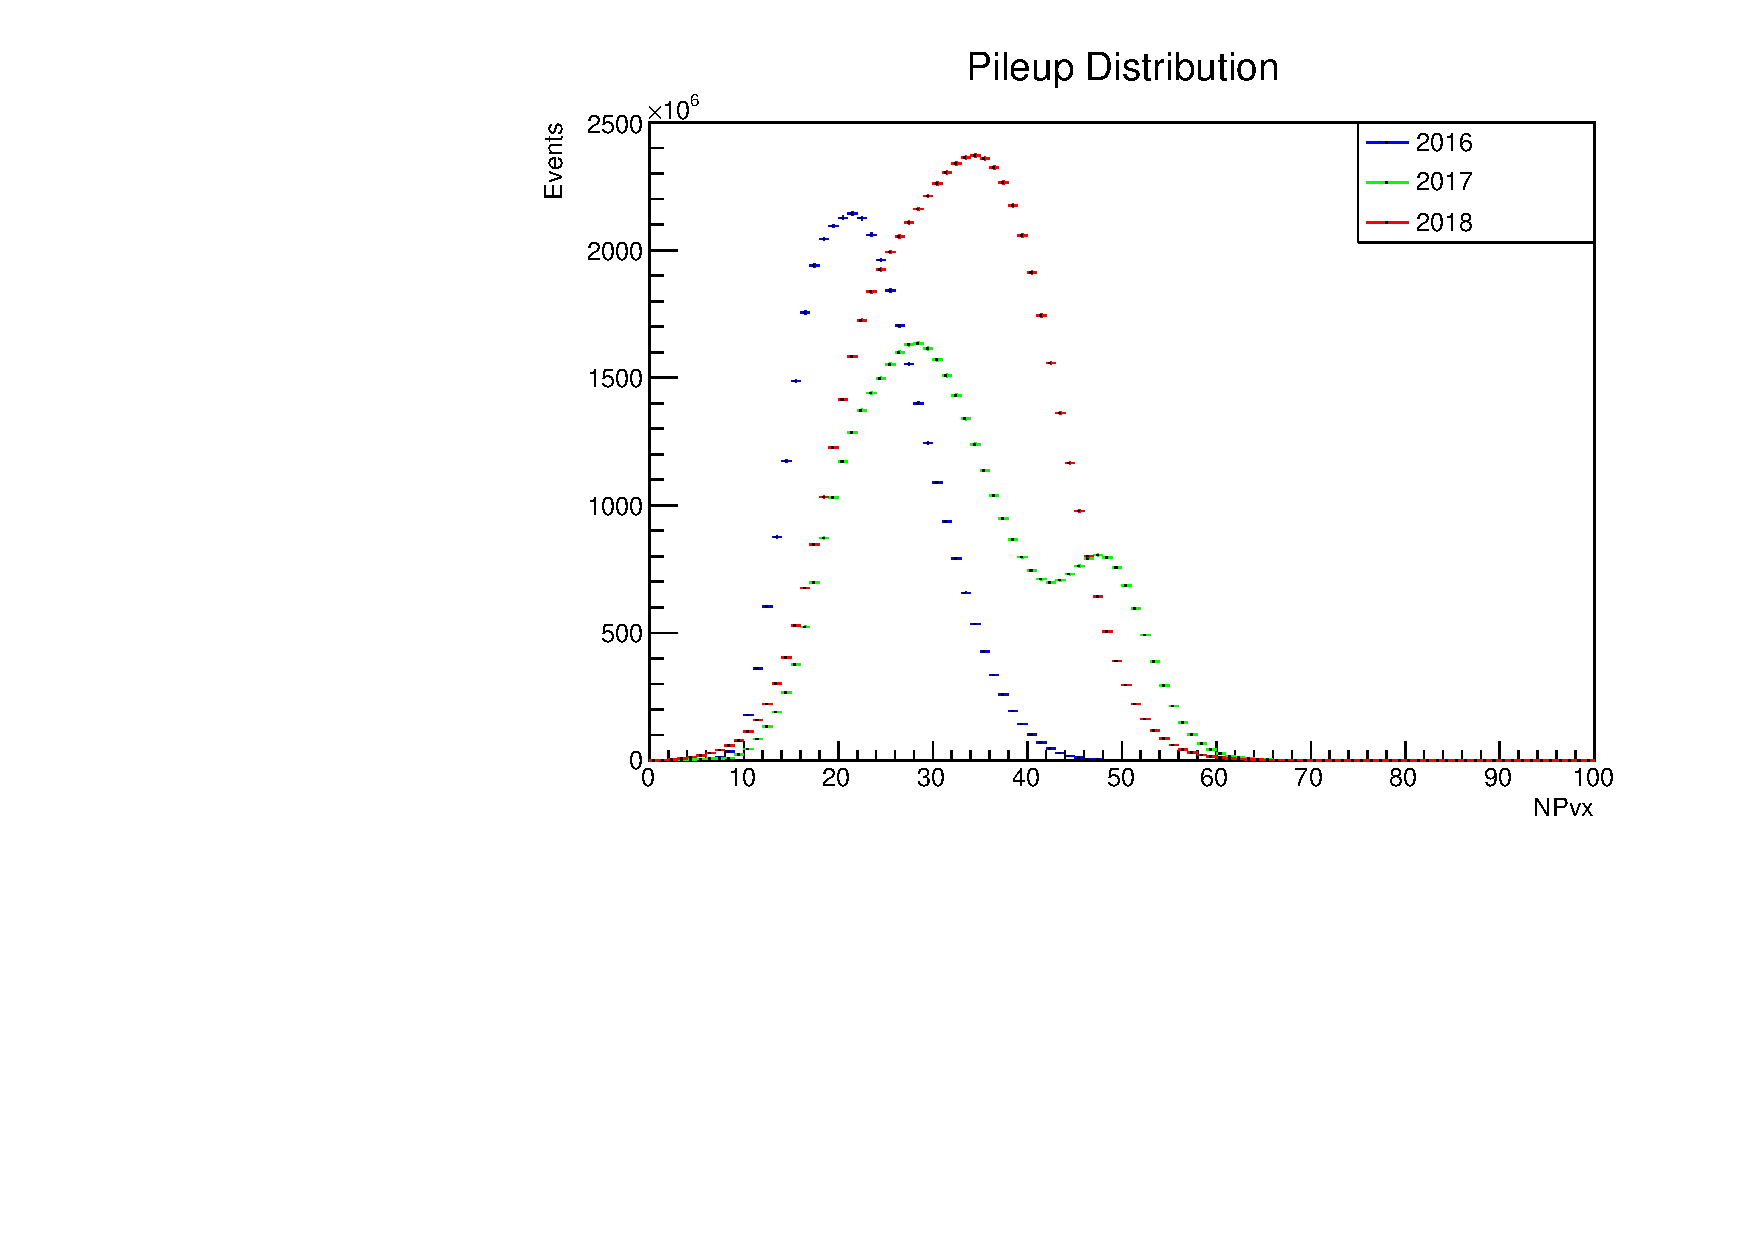
\includegraphics[width=.5\textwidth]{fig/ScaleFactors/GoldenPileup_Linear.pdf}}
        \vfil
        \subfigure[Pileup profile from RunII Data, Logarithmic Scale]{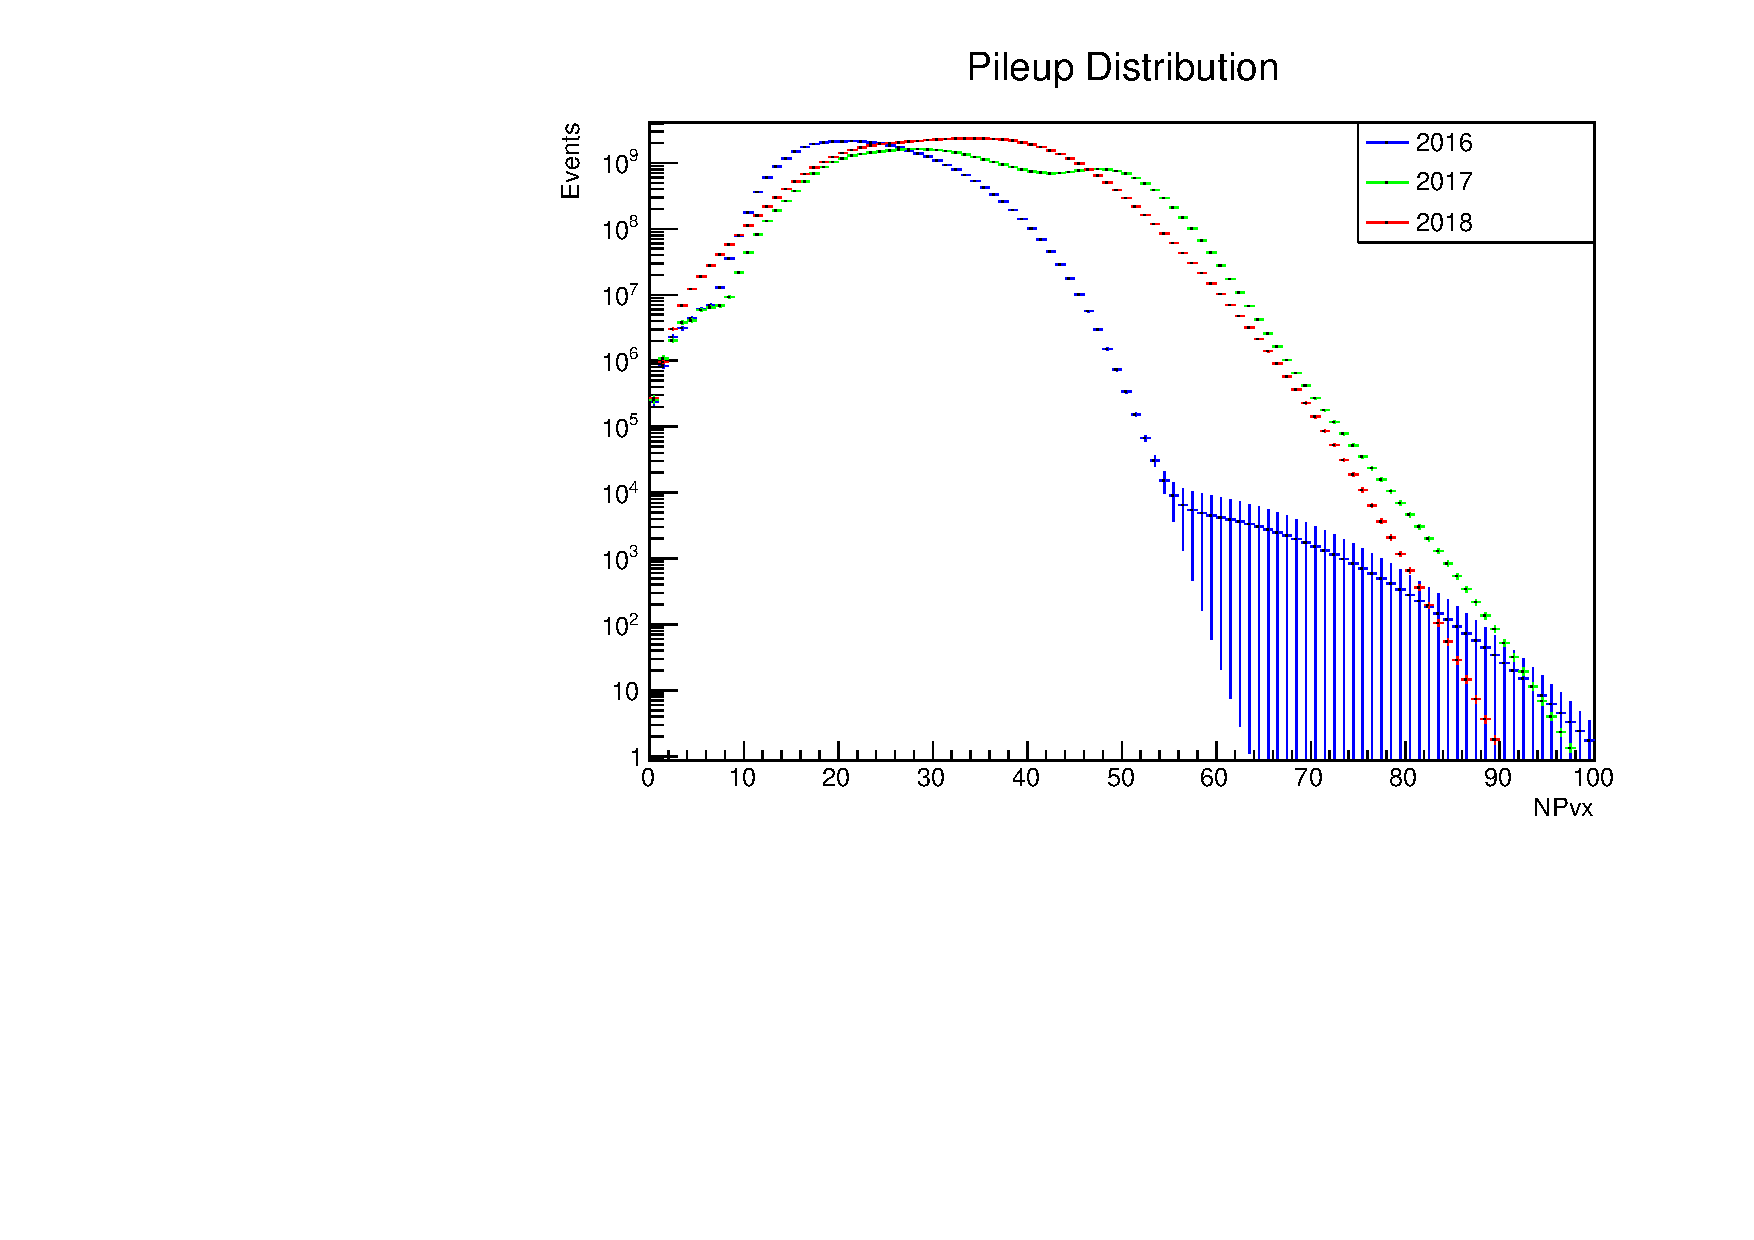
\includegraphics[width=.6\textwidth]{fig/ScaleFactors/GoldenPileup_LogScale.pdf}}
  \caption{Pileup profile distributions for MC and Data}
  \label{fig:RunII_PileupProfiles}
\end{figure}

The number of reconstructed primary vertices in each collision during a period
of time generates a distribution commonly referred as pileup. Montecarlo simulations
are produced with an estimated pileup profile and a correction is needed
in order to match the distributions obtained in the collected data. 
MC Samples are reweighted with $69.2~mb$ as MinBias cross section.
Figure \ref{fig:RunII_PileupProfiles} shows the differences between the
pileup distributions for run 2 data and montecarlo
simulations for the predominant background process (standard model
WZ production). These differences are then
corrected by computing a pileup weight bin by bin that matches the normalized
distribution from montecarlo with the normalized distribution from data.
The normalization of each distribution is eachieved by scaling it by a factor
equivalent to the the inverse of its integral. Each MC event is then reweighted
with the appropiate factor based on the number of reconstructed primary vertices. 

\begin{figure}[tph]
  \centering
        \subfigure[Electron Loose ID]{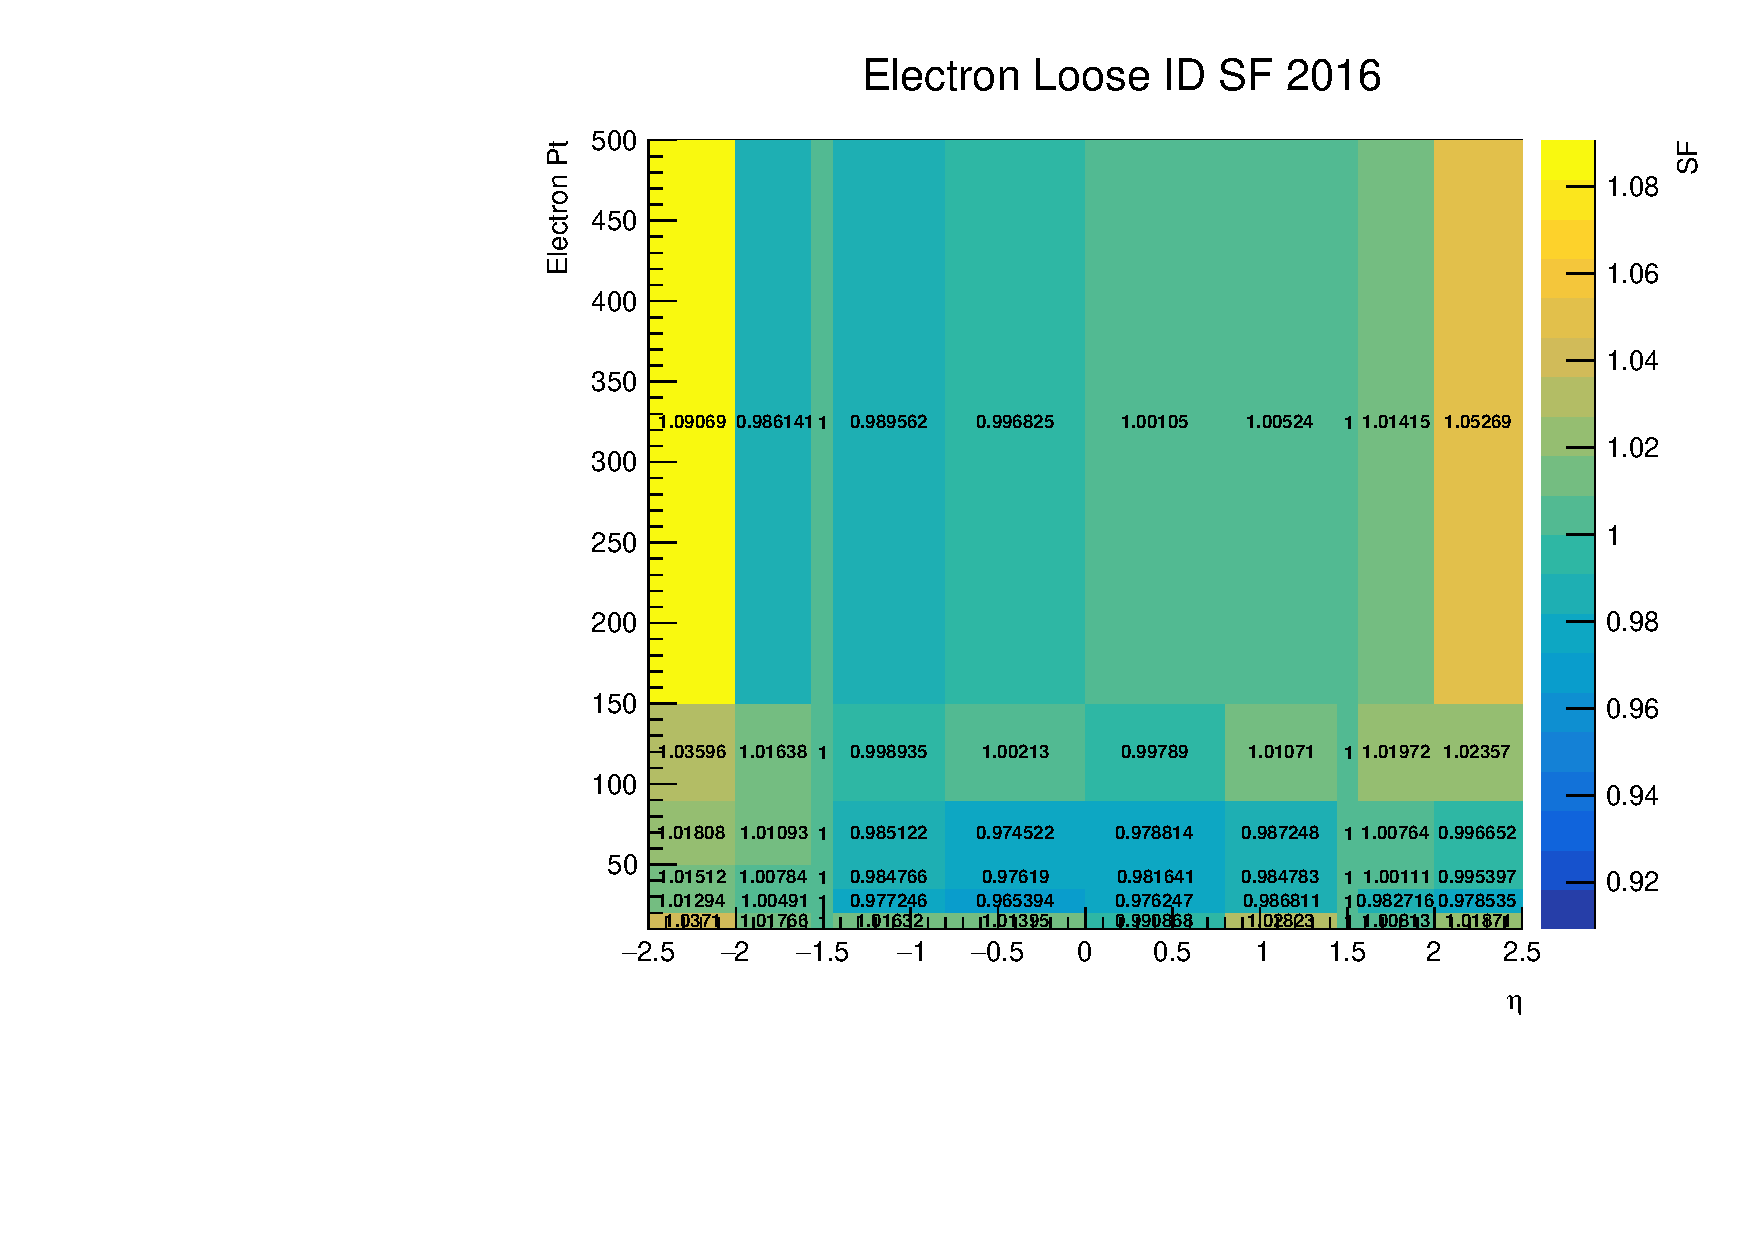
\includegraphics[width=.28\textwidth]{fig/2016Electron_LooseID.pdf}}
        \subfigure[Muon GlobalHighPtId]{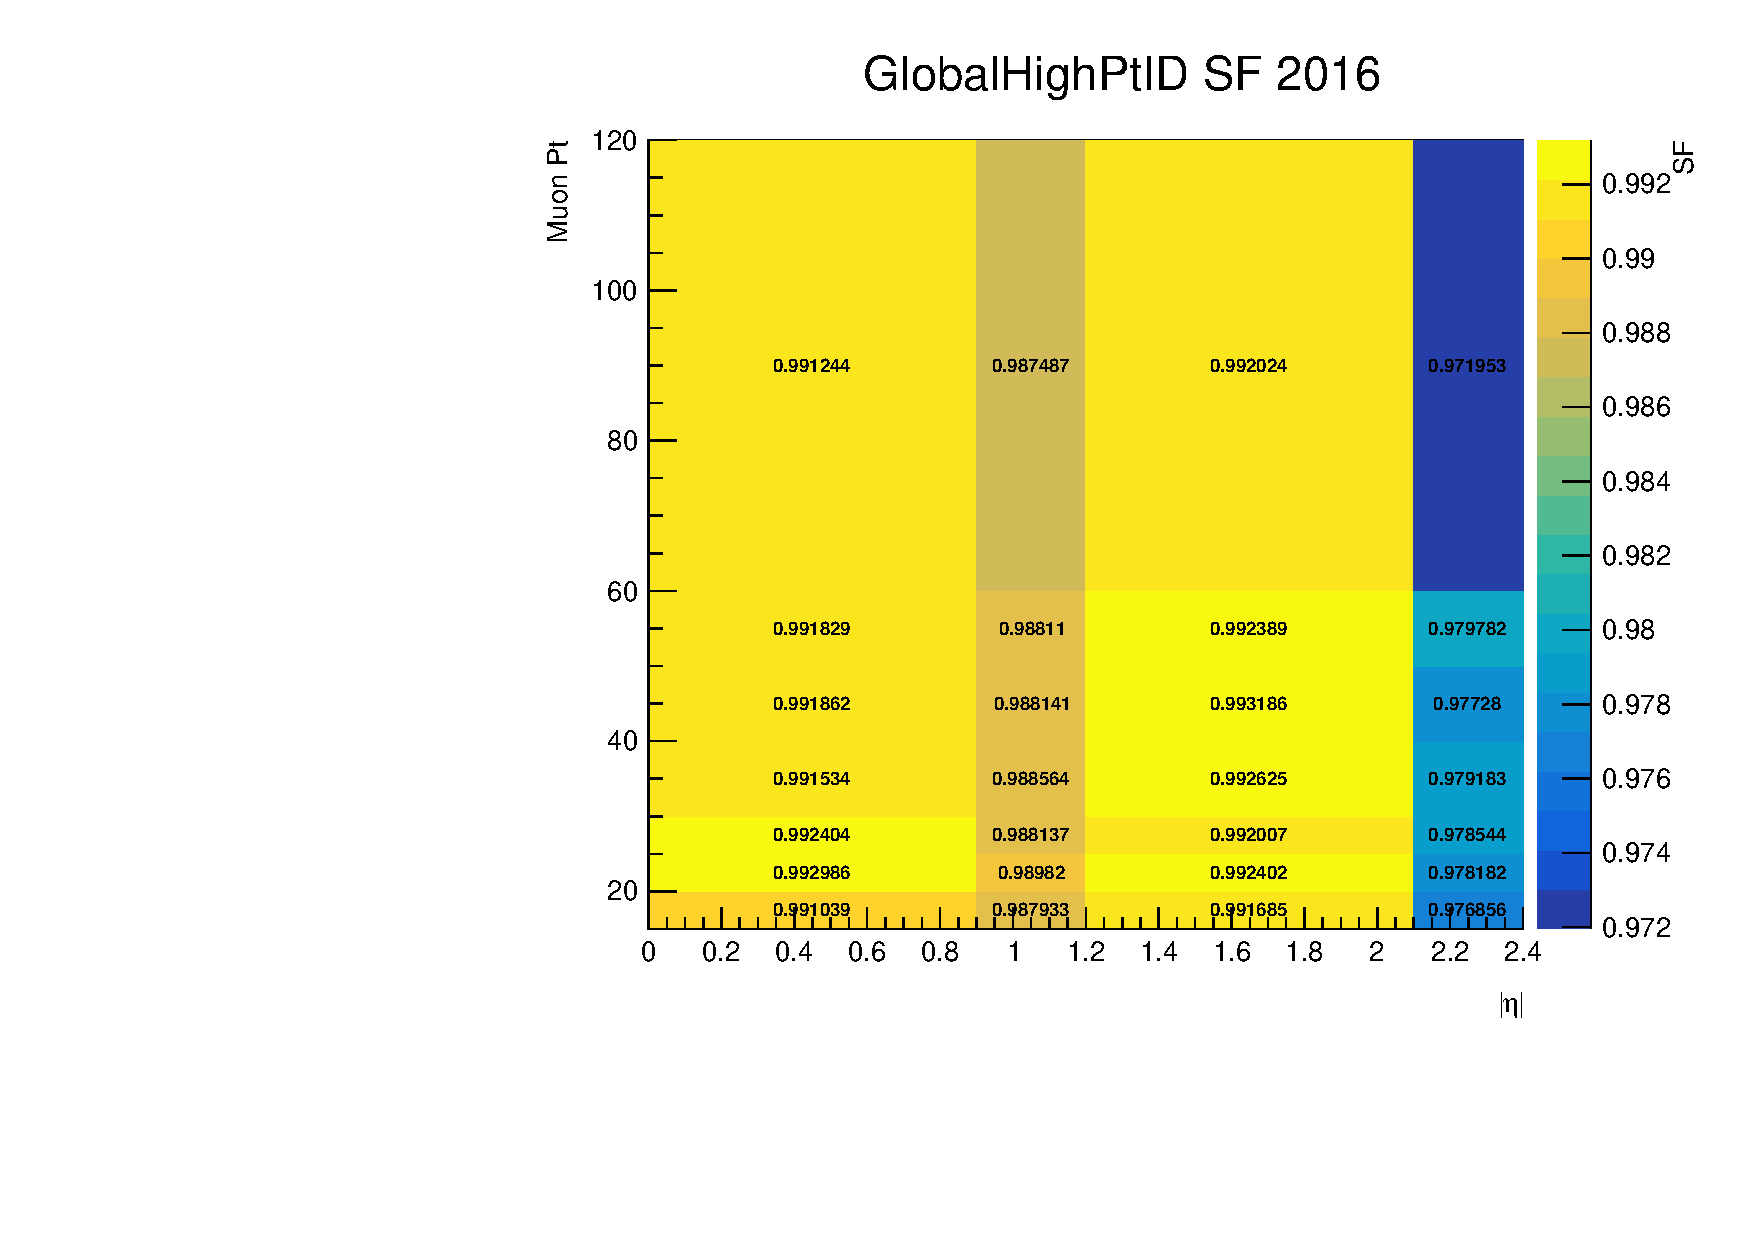
\includegraphics[width=.28\textwidth]{fig/2016Muon_GlobalHighPtID.pdf}}
        \subfigure[Muon TrkHighPtId]{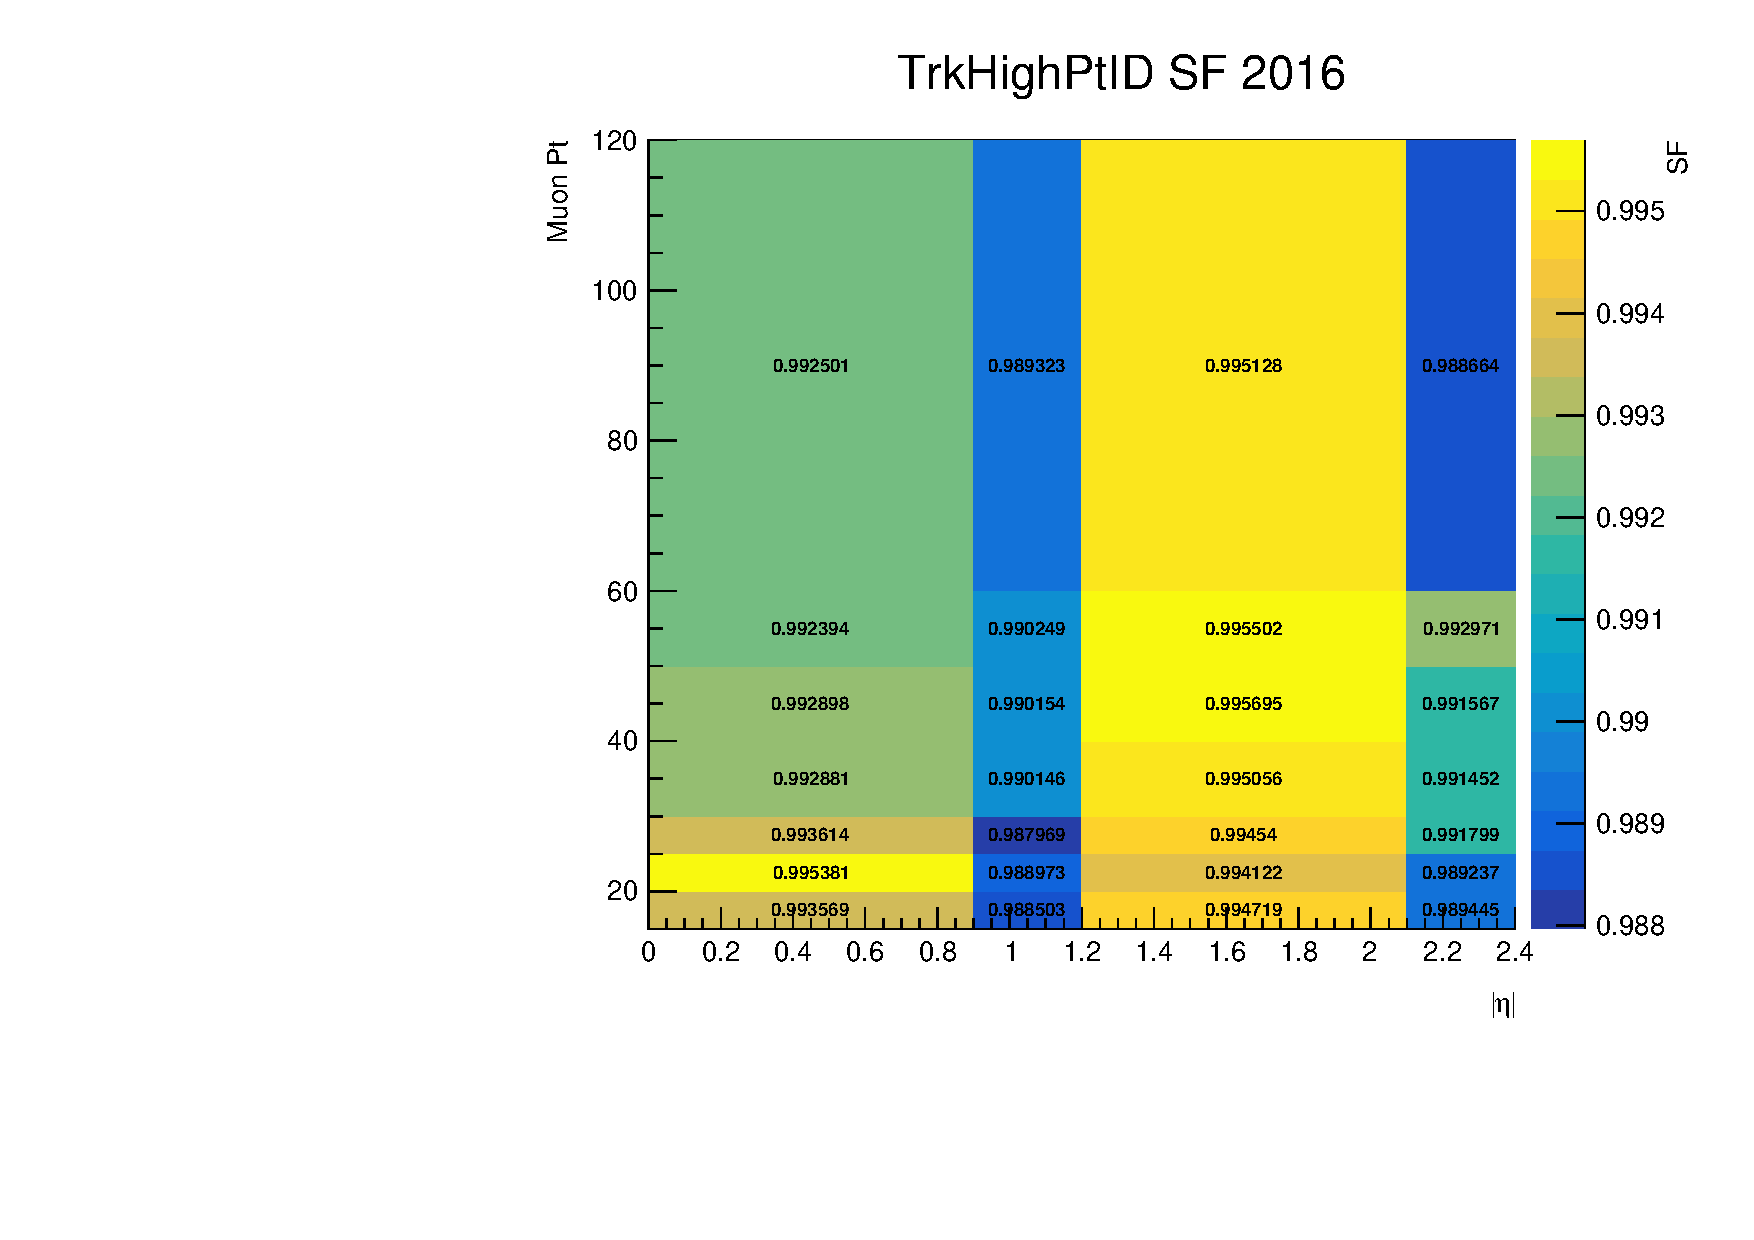
\includegraphics[width=.28\textwidth]{fig/2016Muon_TrkHighPtID.pdf}}
  \caption{SF for different lepton ids}
  \label{fig:leptonidsf}
\end{figure}


\subsection{Lepton scale factors}

Trigger and lepton identification efficiencies are different between data
and montecarlo.

